\documentclass[11pt]{article}

\usepackage[margin=1.05in]{geometry}
\usepackage{amsmath,amssymb,amsthm}
\usepackage{mathtools}
\usepackage{graphicx}
\usepackage{booktabs}
\usepackage{array}
\usepackage{microtype}
\usepackage{xcolor}
\usepackage{tikz}
\usepackage[shortlabels]{enumitem}
\usepackage[colorlinks=true,linkcolor=blue!45!black,citecolor=blue!45!black,urlcolor=blue!45!black]{hyperref}
\hypersetup{pdftitle={Kagey's board in the plane: endpoint crossings for the planar persistent walk},pdfauthor={Arjun Pemmasani}}

% ---------- theorem environments ----------
\newtheorem{theorem}{Theorem}[section]
\newtheorem{lemma}[theorem]{Lemma}
\newtheorem{proposition}[theorem]{Proposition}
\newtheorem{corollary}[theorem]{Corollary}
\theoremstyle{definition}
\newtheorem{definition}[theorem]{Definition}
\newtheorem{example}[theorem]{Example}
\theoremstyle{remark}
\newtheorem{remark}[theorem]{Remark}

% ---------- notation macros ----------
\newcommand{\Z}{\mathbb{Z}}
\newcommand{\R}{\mathbb{R}}
\newcommand{\E}{\mathbb{E}}
\newcommand{\Prob}{\mathbb{P}}
\newcommand{\Var}{\operatorname{Var}}
\newcommand{\Cov}{\operatorname{Cov}}
\newcommand{\supp}{\operatorname{supp}}
\newcommand{\ones}{\mathbf{1}}
\newcommand{\tree}{\operatorname{tree}}
\newcommand{\arb}{\operatorname{arb}}

\graphicspath{{figures/}{../figures/}}

\title{Kagey's board in the plane:\\ endpoint crossings for the planar persistent walk}
\author{Arjun Pemmasani\\[2pt]
 \small Department of Mathematics, Harvey Mudd College\\
 \small Claremont, CA 91711, USA\\
 \small \texttt{apemmasani@hmc.edu}}
\date{}
\begin{document}
\maketitle

\begin{abstract}
A ball bounces down a Galton board with $N$ rows, and each bounce repeats the
previous one with probability $p$. Kagey asked when the middle bin becomes as
likely as an end bin, which only the ball that never switches can reach. We
ask the same question for Kagey's board in the plane, a ball on the square lattice that keeps
its direction, turns left or right, or reverses. For an even number of steps its far corner and
the origin are
equally likely at exactly one switching rate, which we find to first order.
When the ball reverses more often than it turns, this crossing agrees with the
one on Kagey's board with $N/2$ rows, up to a negative power of $N$. When it
turns more often, the crossing comes from a local limit theorem in two
dimensions. On one curve of rates the planar walk is exactly two independent
copies of Kagey's board, and with turns only its crossing is Kagey's up to a
small error.
\end{abstract}

\medskip
\noindent\textbf{Keywords:} persistent random walk; correlated random walk;
Galton board; planar random motion; telegraph process; local limit theorem.

\noindent\textbf{MSC2020:} 60G50; 60F05; 60J10; 60K35.

\section{Introduction}\label{sec:intro}

A ball falls through a Galton board with $N$ rows of pegs. At the first peg it
goes left or right with probability $\frac12$. At every later peg it repeats
its previous direction with probability $p$ and switches with probability
$q=1-p$. Problem~131 of Kagey's Open Problem Collection~\cite{kagey131} asks
for the law of the bin where the ball lands, and in particular when the middle
bin is exactly as likely as an endpoint. An endpoint is reached by a single
path, the one that never switches, so it has probability $\frac12p^{N-1}$. When
$p$ is close to $1$ this path wins, and when $p$ is smaller the middle wins.
Paper~A~\cite{paperA} answers the question at every $N$. The two are equally
likely when the expected number of switches $Nq$ is close to $\log N$. More
precisely, the crossing value $z_N$ of $Nq$ satisfies
$z_N+\frac12\log z_N=\log N+\frac12\log\frac\pi8+o(1)$.

Kagey also asks what changes on other boards. This paper answers his main
question, when the middle is as likely as the ends, for Kagey's board in
two dimensions. A ball moves on the square lattice $\Z^2$, one step east,
north, west or south at a time. It starts in a uniform direction, and at each
step it keeps its direction, turns left or right, or reverses. Turns and
reversals are rare. Fix $T>0$. A turn to each side has probability $rT/N$ and a reversal
has probability $sT/N$, where $r,s\ge0$ are fixed rates with $2r+s>0$. After
$N$ steps, is the ball more likely to be at the corner $(N,0)$, which only the
path that never switches can reach, or back at the origin
(Figure~\ref{fig:planarpaths})? We show that for
every even $N\ge4$ there is exactly one value $T^*_N$ of $T$ at which the two
are equally likely (Proposition~\ref{prop:decomp}). The corner is more likely
below it and the origin above it, and as $N\to\infty$ through even integers
\begin{equation}\label{eq:intro-limit}
 \frac{T^*_N}{\log N}\to\min\Bigl(\frac2{2r+s},\frac1s\Bigr)
\end{equation}
(Theorems~\ref{thm:planar-first} and~\ref{thm:planar-rev}). The two values in
the minimum belong to two kinds of paths to the origin.

\emph{Why two values.} Paper~C~\cite{paperC} gives a rule for a ball with any finite number of
directions. Call a set of directions a face. If the ball makes about $\tau\log N$ switches, the
most likely bin that uses exactly the directions of a face $F$ has probability about
$N^{-\tau\lambda_F-(\lvert F\rvert-1)}$, where $\lambda_F$ is the rate at which the direction
leaves $F$. The first term is the cost of never leaving $F$, and the second is the cost of
sharing the mass of $F$ among about $N^{\lvert F\rvert-1}$ bins.
The planar walk fits this picture. The corner is the face of the single
direction east, with exit rate $2r+s$, so it has probability about
$N^{-(2r+s)\tau}$. A path to the origin either stays on one axis, a face of
two directions with exit rate $2r$, or uses all four directions, a face with exit
rate $0$. On an axis the origin is a single bin of that face, of probability about
$N^{-(2r\tau+1)}$. With all four directions a single bin of the face has
probability about $N^{-3}$, but about $N/2$ of them end at the origin, which
gives $N^{-2}$. This suggests that the origin beats the corner when
$(2r+s)\tau>\min(2r\tau+1,2)$, which is~\eqref{eq:intro-limit}. It is only a
heuristic, since the origin is not a single bin of the full face, and
Section~\ref{sec:planar} proves the limit directly.

\emph{Second order.} The mass at
the origin splits exactly into the paths that stay on one axis and the paths
that use all four directions (Proposition~\ref{prop:decomp}). When reversals
dominate ($s>2r$) the axis paths carry the origin mass at the crossing. Then
$sT^*_N=z_{N/2}+O(N^{-\gamma})$ for some $\gamma>0$, where $z_{N/2}$ is the
crossing of Kagey's board with $N/2$ steps (Theorem~\ref{thm:planar-rev}).
When turns dominate ($s<2r$) the paths with all four directions carry it.
Their mass is given by a local limit theorem in two dimensions
(Theorem~\ref{thm:fourdir}), and the crossing then satisfies
\[
 (2r+s)\,T^*_N+\log T^*_N=2\log N+\log\frac\pi{8(r+s)}+o(1)
\]
(Corollary~\ref{cor:planar-turn}). Here $\log T^*_N$ has the coefficient $1$,
where Kagey's board has $\frac12$, because the origin is a point of a local limit in two
dimensions.

\emph{Two copies of Kagey's board.} There is one curve of switching probabilities on which
everything is exact. If
the walk turns to each side with probability $\rho(1-\rho)$ and reverses with
probability $\rho^2$, its two diagonal coordinates are independent copies of
Kagey's board with switching probability $\rho$. So on this curve the planar
crossing is Kagey's crossing at every $N$ (Proposition~\ref{prop:product}).
With turns only ($s=0$) we show that $rT^*_N=z_N+O((\log N)^2/N)$
(Theorem~\ref{thm:pureturns}).

\subsection{The other papers of the series}\label{sec:series}

This paper is one of six on Problem~131. We call them Paper~A~\cite{paperA},
Paper~B~\cite{paperB}, Paper~C~\cite{paperC}, Paper~D~\cite{paperD}, Paper~E (this paper) and
Paper~F~\cite{paperF}. Paper~A solves Kagey's board. Its uniform Bessel bounds bracket $z_N$
for every $N\ge2$ and give $z_N+\frac12\log z_N=L+c_0+1/(8z_N)+R_N$ with $L=\log N$,
$c_0=\frac12\log(\pi/8)$ and an explicit $R_N$. Paper~B lets the ball switch to
each of $d-1$ other directions at the same rate. Paper~C treats every matrix of switching
rates. It explains which set of directions carries the most likely bin and why, and it locates
the crossings of two such sets. Papers~D and~F ask what
changes when the ball remembers more than its last step.

This paper can be read on its own. From Paper~A we use the run count, the
fact that the bin polynomials grow toward the middle, the uniform Bessel bound
(recalled in~\eqref{eq:planar-bessel}) and the expansion of $z_N$. The proofs do not use
Paper~C, which is the source of the heuristic above.
Figure~\ref{fig:program} compares the crossings of the series.

\begin{figure}[t]
\centering
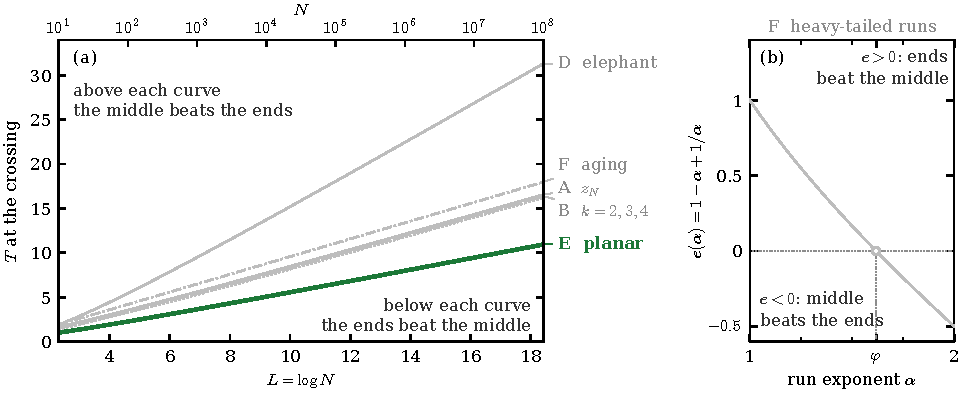
\includegraphics[width=\textwidth]{program_E}
\caption{(a) The crossing on each model's switching scale against $L=\log N$
for the papers of the series. The scale is $T$ for Papers~A, B and~E, $x=N\varepsilon$ for the
elephant walk of Paper~D and the expected number of switches for the aging walk of
Paper~F. The bold curve solves the first crossing equation of
Corollary~\ref{cor:planar-turn} for the planar walk with $r=s=1$, without its
$o(1)$ term. The curve A is $z_N$, and the curves B are the face crossings of
Paper~B.
(b) The exponent $e(\alpha)=1-\alpha+1/\alpha$ of Paper~F for runs with heavy
tails, which changes sign at the golden ratio $\varphi$. (Versions of this
figure also appear in Papers~C, D and~F.)}
\label{fig:program}
\end{figure}

\subsection{Related work}\label{sec:related}

On the lattice the correlated random walk goes back to
Gillis~\cite{gillis1955}. Chen and Renshaw~\cite{chenrenshaw1992} treat the
Gillis--Domb--Fisher walk, and in~\cite{chenrenshaw1994} they show that the
characteristic function of any correlated random walk satisfies a
recurrence. So in principle the law of our planar walk is known. Marris and
Giuggioli~\cite{marris2024} give lattice propagators for walks with forward,
backward and lateral steps. Lenci~\cite{lenci2007} proves recurrence for a
large class of persistent walks on the square lattice. In the continuum, Santra, Basu and
Sabhapandit~\cite{santra2020} find the marginals of a run-and-tumble particle
with four directions, and Angelani~\cite{angelani2022} treats switching among
four orthogonal directions. With turns only, the continuous motion is a
rotation of two independent telegraph processes (Cinque and
Orsingher~\cite[Theorem~2.2]{cinqueorsingher2023}, who credit
Orsingher~\cite{orsingher2000} for constant rates, and Smith, Le Doussal,
Majumdar and Schehr~\cite{sldms2022}). With reversals the two processes are
no longer independent~\cite[Section~3]{cinqueorsingher2023}.
Proposition~\ref{prop:product} is a lattice form of this, and on the lattice
the independent case does have reversals. In the continuum the corners carry
atoms and the origin does not (it has a density in the plane, and with
reversals also along the axes~\cite{kolesnikorsingher2002}), so the comparison
of a corner with the origin is a lattice question. We did
not find the planar crossing of the corner
and the origin in the literature.

\subsection{Plan of the paper}\label{sec:plan}

Section~\ref{sec:notation} fixes the notation and recalls what we use from Paper~A.
Section~\ref{sec:planar} treats the planar walk for general rates. It splits the origin mass,
proves the first-order answer, and locates the crossing when reversals dominate and when turns
dominate. Section~\ref{sec:product} treats the product curve and the walk with turns only.
Section~\ref{sec:verify} describes the computer checks and the open questions, and
Appendix~\ref{app:planar} has the longer proofs.

\section{Notation and the line walk}\label{sec:notation}

This section fixes the notation for the line walk and recalls its crossing equation
from~\cite{paperA}. The planar walk itself is set up at the start of Section~\ref{sec:planar}.

\emph{The line walk.} For $a,b\ge1$ let $S_{a,b}(u)=\sum_wu^{\mathrm{sw}(w)}$, the sum
over the words $w$ with $a$ right steps and $b$ left steps, where $\mathrm{sw}(w)$ is the
number of switches of $w$. Each such word has probability
$\frac12p^{N-1}(q/p)^{\mathrm{sw}(w)}$ under the line walk with $N=a+b$ steps, and we say
that it ends in bin $a$. So
$S_{a,b}(q/p)$ is the probability of bin $a$ divided by the probability
$\frac12p^{N-1}$ of an endpoint. For $N\ge2$ let
$S_N=S_{\lfloor N/2\rfloor,\lceil N/2\rceil}$, which belongs to a middle bin.
It is a nonzero polynomial with nonnegative coefficients
and no constant term, so $S_N(u)=1$ has exactly one positive root $u_N$ (the crossing value of
the odds $u=q/p$ of a switch), and
$p_N=1/(1+u_N)$ is the crossing of the middle and the endpoints. Put $L=\log N$,
$z_N=N(1-p_N)$ and $c_{\mathrm A}=\frac12\log(\pi/8)$. By~\cite{paperA}, $z_N$ satisfies the crossing
equation $z_N+\frac12\log z_N=L+c_{\mathrm A}+1/(8z_N)+R_N$ with an explicit remainder
$R_N=O(1/L^2)$.

\emph{Conventions.} The rates $r$ and $s$ are fixed. Unless we say otherwise, every constant,
every implied constant in $O(\cdot)$ and every threshold for $N$ depends only on them. Limits
and $o(\cdot)$ refer to $N\to\infty$ through even integers. For a path of the planar walk we
write $n_j$ for its number of steps in the direction $j$, and we call the vector
$n=(n_0,n_1,n_2,n_3)$ its composition.

\section{The planar persistent walk}\label{sec:planar}

We now set up the planar persistent walk. It moves on $\Z^2$ in the directions east, north, west and
south, numbered $0,1,2,3$ modulo $4$, with unit vectors $e_0=(1,0)$, $e_1=(0,1)$,
$e_2=-e_0$ and $e_3=-e_1$. Let $r,s\ge0$ with $\beta=2r+s>0$, and let
$0<h<1/\beta$. The first direction is uniform. After that the walk keeps its
direction with probability $p_0=1-\beta h$, turns left or right with
probability $rh$ each, and reverses with probability $sh$. In the notation
of~\cite{paperC} the direction is the chain with the rates $q_{j,j\pm1}=r$ and
$q_{j,j+2}=s$. The
position after $N$ steps is $Y_N=(n_0-n_2,n_1-n_3)$. So $Y_N$ is a linear
function of the composition. Throughout, $N$ is even, since otherwise the
origin cannot be reached. We write $T=Nh$. Only
the path that always goes east reaches the corner $Ne_0$, so
\[
 c_N=\Prob(Y_N=Ne_0)=\tfrac14p_0^{N-1}.
\]
We compare it with $o_N=\Prob(Y_N=0)$. Figure~\ref{fig:planarpaths} shows the
three kinds of paths that matter.

\begin{figure}[t]
\centering
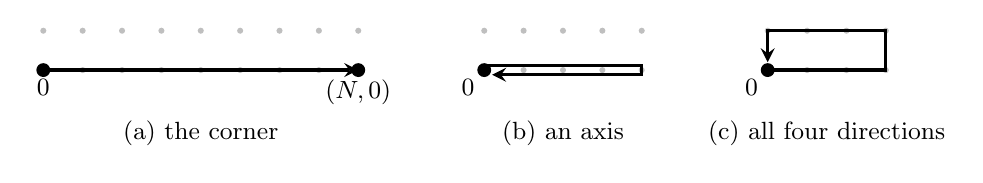
\begin{tikzpicture}[x=0.5cm,y=0.5cm,font=\small,>=stealth]
 \foreach \x in {0,...,8} \foreach \y in {0,1} \fill[gray!50] (\x,\y) circle (1.1pt);
 \draw[very thick,->] (0,0) -- (8,0);
 \fill (0,0) circle (2.5pt) node[below] {$0$};
 \fill (8,0) circle (2.5pt) node[below] {$(N,0)$};
 \node at (4,-1.6) {(a) the corner};
 \begin{scope}[xshift=5.6cm]
 \foreach \x in {0,...,4} \foreach \y in {0,1} \fill[gray!50] (\x,\y) circle (1.1pt);
 \draw[very thick,->] (0,0.12) -- (4,0.12) -- (4,-0.12) -- (0.2,-0.12);
 \fill (0,0) circle (2.5pt) node[below left] {$0$};
 \node at (2,-1.6) {(b) an axis};
 \end{scope}
 \begin{scope}[xshift=9.2cm]
 \foreach \x in {0,...,3} \foreach \y in {0,1} \fill[gray!50] (\x,\y) circle (1.1pt);
 \draw[very thick,->] (0,0) -- (3,0) -- (3,1) -- (0,1) -- (0,0.2);
 \fill (0,0) circle (2.5pt) node[below left] {$0$};
 \node at (1.5,-1.6) {(c) all four directions};
 \end{scope}
\end{tikzpicture}
\caption{Paths of $N=8$ steps. (a) The only path to the corner $(N,0)$ never
switches. A path to the origin either (b) stays on one axis and only reverses,
or (c) turns and then uses all four directions.}
\label{fig:planarpaths}
\end{figure}

We write $u=sh/p_0$, $v=rh/p_0$ and $w=\beta h/p_0=2v+u$, so $1+w=1/p_0$. These
are the odds of a reversal, of a turn to a given side and of any switch, as in
the notation $u=q/p$ of Section~\ref{sec:notation}. We use $S_N$, $u_N$, $p_N$, $z_N=N(1-p_N)$ and
$c_0$ from Section~\ref{sec:notation}. As $N$ is even, $S_N(u)$ is the sum of
$u^j$ over the words with $N/2$ letters of each of two kinds, where $j$ is the
number of switches. It has nonnegative coefficients and no constant term, so it
increases strictly on $[0,\infty)$.

\emph{The answer at first order.} The face selection of~\cite{paperC} predicts the answer, up to
powers of $\log N$, as in the introduction. Let $h=\tau\log N/N$. The corner is the vertex $\{0\}$,
which has exit rate $\beta$, so $c_N$ is about $N^{-\beta\tau}$. A vertex, a
face with three directions, or a face with two adjacent ones misses the opposite of
one of its directions, so it cannot reach the origin. On the axis $\{0,2\}$,
which has exit rate $2r$, the origin is the single composition
$(N/2,0,N/2,0)$, of probability about $N^{-(2r\tau+1)}$. On the full face a
single composition has probability about $N^{-3}$, but about $N/2$
compositions $(a,b,a,b)$ end at the origin, and together they give about
$N^{-2}$. So the origin should beat the corner when $\beta\tau>\min(2r\tau+1,2)$,
that is, when $\tau>\tau^*=\min(2/\beta,1/s)$, with $1/0=\infty$. At $\tau^*$ the axes win if
$s>2r$ and the full face wins if $s<2r$. This is only a heuristic, since it
applies the first-order face selection of~\cite{paperC} to a linear function of the composition, and no such rule
is proved in general.

The rest of the section proves this and then locates the crossing. We split
the origin mass into an axis part and a part with all four directions
(Proposition~\ref{prop:decomp}) and prove the first-order answer
(Theorem~\ref{thm:planar-first}). Then we find the crossing up to
$O(N^{-\gamma})$ when reversals dominate (Theorem~\ref{thm:planar-rev}) and up
to $o(1)$ when turns dominate (Theorem~\ref{thm:fourdir} and
Corollary~\ref{cor:planar-turn}). Section~\ref{sec:product} treats two cases in
which the walk is, exactly or nearly, two copies of the line walk.

\emph{Three levels.} A path is given by the number of times it switches, the
directions of its runs, and the lengths of its runs.

\begin{lemma}[three levels]\label{lem:threelevel}
Write a sequence of directions as its number $m$ of switches, its skeleton $Z=(Z_0,\dots,Z_m)$,
which lists the directions of the runs so that $Z_t\ne Z_{t-1}$, and its run lengths
$\ell=(\ell_0,\dots,\ell_m)$, which form a composition of $N$ into $m+1$ positive parts. This is a
bijection, and $Y_N=\sum_{t=0}^m\ell_te_{Z_t}$. Under the walk, \textup{(a)} $m$ has the law
$\mathrm{Bin}(N-1,\beta h)$. Given $m$, \textup{(b)} $Z$ and $\ell$ are independent, \textup{(c)}
$Z$ is the random walk on $\Z_4$ with uniform $Z_0$ whose independent increments are $\pm1$ with
probability $r/\beta$ each and $2$ with probability $s/\beta$, and \textup{(d)} $\ell$ is uniform on
the $\binom{N-1}m$ compositions.
\end{lemma}

\begin{proof}
We write down the probability of one sequence and factor it. The map is a bijection because the
runs of a sequence determine $(m,Z,\ell)$ and are determined by it. Put $\lambda(\pm1)=r$ and $\lambda(2)=s$.
A sequence with data $(m,Z,\ell)$ starts in the direction $Z_0$ with probability $\frac14$, keeps
its direction at $N-1-m$ steps, and makes the switch from $Z_{t-1}$ to $Z_t$ with probability
$h\,\lambda(Z_t-Z_{t-1})$. So it has probability
\[
 \frac14p_0^{N-1-m}\prod_{t=1}^mh\,\lambda(Z_t-Z_{t-1})
 =\binom{N-1}m(\beta h)^mp_0^{N-1-m}\cdot\frac14\prod_{t=1}^m\frac{\lambda(Z_t-Z_{t-1})}\beta
 \cdot\binom{N-1}m^{-1}.
\]
The run lengths do not appear on the left, which is why they are uniform. On the right, the first
factor depends only on $m$. For fixed $m$ the middle factor is the probability of $Z$ under the walk
in (c), so it sums to $1$ over the skeletons, and the last factor sums to $1$ over the
$\binom{N-1}m$ compositions. So the three factors are the laws in (a), (c) and (d), and the product
form gives (b).
\end{proof}

The next proposition separates the skeletons that stay on one axis from those
that use both.

\begin{proposition}[exact decomposition and a unique crossing]\label{prop:decomp}
Let $N\ge2$ be even and $0<h<1/\beta$. Let $o^{(0)}_N$ and $o^{(4)}_N$ be the probabilities that
$Y_N=0$ and the walk never turns, and that $Y_N=0$ and the walk uses all four directions. Then
$o_N=o^{(0)}_N+o^{(4)}_N$,
\[
 o^{(0)}_N=2S_N(u)\,c_N,\qquad 0\le o^{(4)}_N\le\frac{w^2}{2p_0}\bigl(1-p_0^N\bigr).
\]
Equivalently, $o_N/c_N=2S_N(u)+E_N$ with $0\le E_N\le2w^2\bigl((1+w)^N-1\bigr)$. Also, $o_N/c_N$
is a polynomial in $v$ and $u$ with nonnegative coefficients and no constant term. If $s>0$, or if
$s=0$ and $N\ge4$, it increases strictly in $h$ from $0$ at $h=0$ to $\infty$ as $h\uparrow1/\beta$.
So there is exactly one $h^*_N\in(0,1/\beta)$ with $o_N=c_N$, and the corner is more likely than the
origin exactly when $h<h^*_N$.
\end{proposition}

In words, the origin mass splits exactly into two parts. The axis part,
measured against the corner, is twice the middle bin of the line walk with
switching odds $u$, measured against its endpoint. The part from paths with all
four directions is small when $w$ is small. The ratio
$o_N/c_N$ grows with the switching rate, so the corner and the origin cross
exactly once, at every even $N\ge4$.

\begin{proof}
We sort the origin paths by whether they turn, and then we write $o_N/c_N$ as a sum over paths.
An origin path with no turn stays on the axis of its first step. An origin path that turns uses both
axes, and since $n_0=n_2$ and $n_1=n_3$ at the origin, it uses all four directions. So every origin
path is of exactly one of the two kinds. The origin paths on the axis $\{0,2\}$ are the paths with
$n_0=n_2=N/2$, and the path that always goes east has probability $c_N$. A path on this axis
with $j$ reversals has probability $\frac14p_0^{N-1-j}(sh)^j=c_Nu^j$. So by the definition of
$S_N$ these paths have total probability $S_N(u)c_N$, and the same holds on the axis $\{1,3\}$.
Hence $o^{(0)}_N=2S_N(u)c_N$. (For a pair of states of a general chain this
identity is proved in~\cite{paperC}.) The bound on $o^{(4)}_N$ follows from Lemma~\ref{lem:threelevel} and a count
of the run lengths that bring a skeleton back to the origin. We prove it in
Appendix~\ref{app:planar}. Dividing by $c_N$ gives the form with $E_N$.

A path with $j$ turns and $k$ reversals has probability $\frac14p_0^{N-1-j-k}(rh)^j(sh)^k=c_Nv^ju^k$.
So $o_N/c_N$ is the sum of $v^ju^k$ over the origin paths, and $j+k\ge1$ for each of them. Both $u$
and $v$ are nondecreasing in $h$, and each of them with a positive rate increases strictly to
$\infty$ as $h\uparrow1/\beta$. If $s>0$, the path that goes east $N/2$ times and then west gives
the term $u$. If $s=0$ and $N\ge4$, then $r>0$, and a path whose four runs go east, north, west and
south, with lengths $\ell_0=\ell_2\ge1$ and $\ell_1=\ell_3\ge1$, gives the term $v^3$. This proves
the claims on monotonicity and the limits. For $s=0$ and $N=2$ the origin cannot be reached.
\end{proof}

The identity and the unique crossing for $s>0$ are also checked in Lean~4 (Section~\ref{sec:verify}). We
write $T^*_N=Nh^*_N$ for the crossing and $u^*_N=sh^*_N/(1-\beta h^*_N)$ for the odds of a reversal
there. At the crossing $o_N=c_N$, so $2S_N(u^*_N)=o^{(0)}_N/o_N$ there. We call this number the
zero-turn share of the origin mass.

We compare $S_N$ with Bessel functions by the uniform Bessel bound
of~\cite[Theorem~3.3(i)]{paperA}. Put $\psi(z)=z(I_0(z)+I_1(z))$. In our notation that bound says
that for every $N\ge2$ (even or odd) and every $z>0$
\begin{equation}\label{eq:planar-bessel}
 \Bigl(1-\frac{z(z+2)}{2N}\Bigr)\psi(z)\le\frac N2\,S_N\Bigl(\frac zN\Bigr)\le\psi(z).
\end{equation}
Since $I_0'=I_1$ and $(zI_1)'=zI_0$, we have $\psi'=\psi+I_0$, so $(\log\psi)'\ge1$. We use this
to turn a bound on $\psi(z)$ into a bound on $z$.

\begin{theorem}[first order]\label{thm:planar-first}
Fix $r>0$ and $s\ge0$, put $\tau^*=\min(2/\beta,1/s)$ with $1/0=\infty$, and let $N\to\infty$
through even integers.
\begin{enumerate}[(a)]
\item Fix $\tau>0$ and put $h=\tau\log N/N$. If $\tau<\tau^*$, then $o_N/c_N\le N^{-\gamma}$ for
some $\gamma>0$ and all large $N$. If $\tau>\tau^*$, then $o_N/c_N\ge N^{\gamma}$ for some
$\gamma>0$ and all large $N$.
\item The ratio $T^*_N/\log N$ tends to $\tau^*$.
\item If $s>2r$, then $2S_N(u^*_N)\to1$, so the origin mass at the crossing comes from the two axes,
half from each. If $s<2r$, then $2S_N(u^*_N)\le N^{-\gamma}$ for some $\gamma>0$ and all large $N$,
so it comes from the paths that use all four directions.
\end{enumerate}
\end{theorem}

In words, the heuristic above gives the right first-order answer. The crossing sits at $T\approx\tau^*\log
N$, and at the crossing the origin is reached through the axes when reversals
dominate and through all four directions when turns dominate. (For $r=0$ the
walk never leaves the axis of its first step, and Theorem~\ref{thm:planar-rev}(c)
gives the same limit $1/s$.)

\emph{Idea of the proof.} The proof is in Appendix~\ref{app:planar}. The upper
bound in (a) follows from Proposition~\ref{prop:decomp} and
\eqref{eq:planar-bessel}. For the lower bound when $s\tau>1$ the axis part is
enough. For the lower bound when $\beta\tau>2$ we count balanced skeletons, those
with as many runs east as west and as many north as south, with
Lemma~\ref{lem:threelevel}. They give $o^{(4)}_N$ of order at least
$N^{-2}T^{-1/2}$. Part (b) follows from (a) and the monotonicity in
Proposition~\ref{prop:decomp}, and part (c) from (b) and the bounds on the two
parts.

\emph{Reversals dominate.} Let $s>2r$. Then the origin mass at the crossing
comes from the axes, and on an axis the walk is the line walk. Up to an error
$O(N^{-\gamma})$ the crossing
is then the crossing of~\cite{paperA} for $N/2$ steps. We write
$z_{N/2}=\frac N2(1-p_{N/2})$ for it, and put
\[
 \mathcal A(\Lambda)=\Lambda-\tfrac12\log\Lambda+c_0
 +\frac{\frac14\log\Lambda-\frac12c_0+\frac18}{\Lambda},
\]
so that the third-order expansion of $z_N$ in~\cite[Corollary~3.7(c)]{paperA} reads
$z_N=\mathcal A(L)+O((\log L)^2/L^2)$.

\begin{theorem}[reversals dominate]\label{thm:planar-rev}
\begin{enumerate}[(a)]
\item Let $s>0$. For all even $N\ge2$ and $0<h<1/\beta$,
\[
 \frac{o_N}{c_N}=2S_N(u)\bigl(1+\varepsilon_N(h)\bigr),\qquad
 0\le\varepsilon_N(h)\le\frac{w^2(1+w)^N}{S_N(u)}.
\]
\item Let $r\ge0$ and $s>2r$, let $N\to\infty$ through even integers, and let
$0<\gamma<1-2r/s$. Then
\[
 \varepsilon_N(h^*_N)=O\bigl((\log N)^{3/2-r/s}N^{-(s-2r)/s}\bigr),\qquad
 Nu^*_N=z_{N/2}+O(N^{-\gamma}).
\]
\item Under the hypotheses of (b), $sT^*_N=z_{N/2}+O(N^{-\gamma})$. Hence
\[
 sT^*_N=\mathcal A(L-\log2)+O\Bigl(\frac{(\log L)^2}{L^2}\Bigr),\qquad
 sT^*_N-z_N=-\log2+\frac{\log2}{2L}+O\Bigl(\frac{(\log L)^2}{L^2}\Bigr).
\]
\end{enumerate}
\end{theorem}

In words, when reversals dominate, the planar walk at its crossing behaves like
the line walk with half as many steps, and $sT^*_N$ is smaller than the
crossing $z_N$ of the line walk by about $\log2$. Here is why. At the crossing $o_N\approx
o^{(0)}_N=2S_N(u)c_N$, so the crossing solves $2S_N(u)\approx1$.
By~\eqref{eq:planar-bessel}, applied with $N$ and with $N/2$ steps, the
equations $2S_N(z/N)=1$ and $S_{N/2}(z/(N/2))=1$ both say that
$\psi(z)\approx N/4$. So doubling $S_N$ has the same effect as halving $N$.

\begin{proof}
(a) Since $s>0$, $S_N(u)\ge2u>0$. Divide Proposition~\ref{prop:decomp} by $2S_N(u)$. Then
$\varepsilon_N(h)=E_N/(2S_N(u))$ and $E_N\le2w^2(1+w)^N$.

(b) The proof has two steps. We first show that the four-direction part $E_N$ is negligible at the
crossing, so that the crossing nearly solves $2S_N(u)=1$. Then we compare this equation with the
equation $S_{N/2}(u)=1$ of the crossing of the line walk for $N/2$ steps. Both equations become statements about
$\psi$, and $\psi$ grows so fast that nearly equal values force nearly equal arguments. Write
$u^*=u^*_N$ and $z^*=Nu^*$, and let $E^*$ be the value of $E_N$ at $h=h^*_N$.

\emph{Step 1 ($E^*$ is small).} At the crossing $o_N/c_N=1$, so Proposition~\ref{prop:decomp} gives
\[
 2S_N(u^*)+E^*=1.
\]
Hence $S_N(u^*)\le\frac12<1=S_N(u_N)$, and $u^*<u_N$ because $S_N$ is increasing. Now
$w=\beta u/s$ for every $h$, so the value of $w$ at the crossing is below $w_N=\beta u_N/s$. The
bound $E_N\le2w^2(1+w)^N$ of Proposition~\ref{prop:decomp} increases with $w$, so
\[
 E^*\le\eta_N:=2w_N^2(1+w_N)^N\le2w_N^2e^{Nw_N}.
\]
We estimate $\eta_N$. The second-order expansion of $z_N$
in~\cite[Corollary~3.7(b)]{paperA} gives $Nu_N=z_N/p_N=L-\frac12\log L+O(1)$. So
$Nw_N=\frac\beta s(L-\frac12\log L)+O(1)$, and
\[
 e^{Nw_N}=O\bigl(N^{\beta/s}L^{-\beta/(2s)}\bigr),\qquad w_N^2=O\Bigl(\frac{L^2}{N^2}\Bigr).
\]
In the product the exponent of $N$ is $\beta/s-2=-(s-2r)/s$, and the exponent of $L$ is
$2-\beta/(2s)=\frac32-\frac rs$. Hence
\[
 \eta_N=O\bigl(L^{3/2-r/s}N^{-(s-2r)/s}\bigr),
\]
which tends to $0$ because $s>2r$. Since $2S_N(u^*)=1-E^*$, part (a) gives
$\varepsilon_N(h^*_N)=E^*/(1-E^*)\le\eta_N/(1-\eta_N)$. This is the first claim.

\emph{Step 2 (comparison with $N/2$ steps).} Let $z'=\frac N2u_{N/2}$, so that
$S_{N/2}(z'/(N/2))=1$. We apply \eqref{eq:planar-bessel} twice. With $N/2$ steps at $z'$ it reads
$(1-\delta'_N)\psi(z')\le\frac N4\le\psi(z')$, where $\delta'_N=z'(z'+2)/N$. With $N$ steps at $z^*$
it reads $(1-\delta_N)\psi(z^*)\le\frac N2S_N(u^*)\le\psi(z^*)$, where
$\delta_N=z^*(z^*+2)/(2N)$, and Step 1 gives $\frac14(1-\eta_N)\le\frac12S_N(u^*)\le\frac14$.
Together,
\[
 \frac N4\le\psi(z')\le\frac N4\cdot\frac1{1-\delta'_N},\qquad
 \frac N4(1-\eta_N)\le\psi(z^*)\le\frac N4\cdot\frac1{1-\delta_N}.
\]
So $\psi$ is close to $N/4$ at both points. Both $z'$ and $z^*<Nu_N$ are $O(L)$, so $\delta_N$ and
$\delta'_N$ are $O(L^2/N)$, and taking logarithms gives
$\lvert\log\psi(z^*)-\log\psi(z')\rvert=O(\eta_N+L^2/N)$. Since $(\log\psi)'\ge1$, two points are
never farther apart than their values of $\log\psi$. So
\[
 \lvert z^*-z'\rvert\le\lvert\log\psi(z^*)-\log\psi(z')\rvert=O\Bigl(\eta_N+\frac{L^2}N\Bigr).
\]
Finally $z_{N/2}=\frac N2(1-p_{N/2})=z'/(1+u_{N/2})$ and $u_{N/2}=O(L/N)$, so
$z_{N/2}=z'+O(L^2/N)$. Hence $z^*-z_{N/2}=O(\eta_N+L^2/N)$. By the bound on $\eta_N$ in Step 1
this is $O(N^{-\gamma})$, because $\gamma<1-2r/s$.

(c) We pass from $Nu^*_N$ to $sT^*_N$ and then insert the expansion of $z_N$. Since
$u=sh/(1-\beta h)$, we have $h^*_N=u^*/(s+\beta u^*)$. So $sT^*_N=z^*/(1+\beta u^*/s)=z^*+O(L^2/N)$, as
$u^*<u_N=O(L/N)$. With (b) this gives $sT^*_N=z_{N/2}+O(N^{-\gamma})$. The third-order expansion of
$z_N$, for $N/2$ steps and for $N$ steps, gives
$z_{N/2}=\mathcal A(L-\log2)+O((\log L)^2/L^2)$ and $z_N=\mathcal A(L)+O((\log L)^2/L^2)$, since
$\log(N/2)=L-\log2$. This is the first display. For the second we subtract. The last
term of $\mathcal A$ has derivative $O(\log L/L^2)$ near $L$, so
\[
 \mathcal A(L-\log2)-\mathcal A(L)=-\log2-\tfrac12\log\Bigl(1-\frac{\log2}L\Bigr)
 +O\Bigl(\frac{\log L}{L^2}\Bigr)=-\log2+\frac{\log2}{2L}+O\Bigl(\frac{\log L}{L^2}\Bigr).
\qedhere
\]
\end{proof}

For $(r,s)=(0.1,1)$ a numerical computation of the exact law gives the difference $sT^*_N-z_N$ as $-0.6317$ at $N=640$ and $-0.6493$ at
$N=10240$, while the first two terms in (c) give $-0.6395$ and $-0.6556$ (Figure~\ref{fig:planar}(a)).

\begin{figure}[t]
\centering
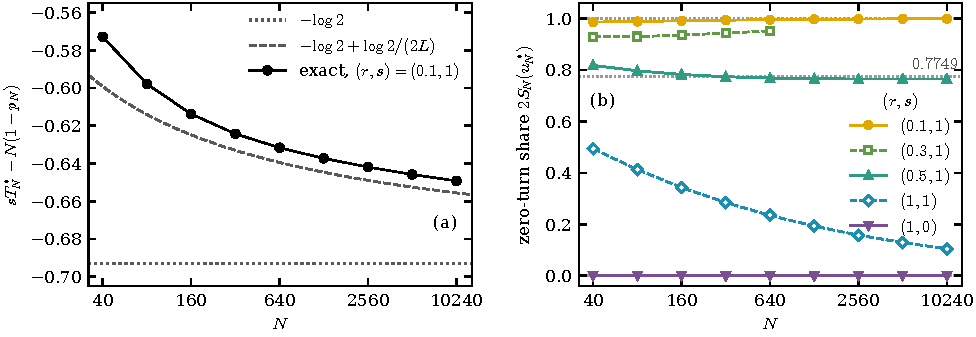
\includegraphics[width=\textwidth]{fig_planar}
\caption{(a) The exact crossing of the planar walk with $(r,s)=(0.1,1)$, written as
$sT^*_N-z_N$ with $z_N=N(1-p_N)$, for $N=40\cdot2^k$ with $0\le k\le8$. The dashed curve is
$-\log2+\log2/(2L)$ from Theorem~\ref{thm:planar-rev}(c), and the dotted line is its limit $-\log2$.
(b) The zero-turn share $2S_N(u^*_N)$ of the origin mass at the crossing. It tends to $1$ for
$s>2r$ and to $0$ for $s<2r$ (Theorem~\ref{thm:planar-first}(c)), and to
$2\sqrt2/(\sqrt2+\sqrt5)=0.7749$ at the switch $s=2r$ (Corollary~\ref{cor:planar-turn}(b)). For
$(r,s)=(1,0)$ there are no reversals and the share is $0$ for every $N$. This is the walk with
turns only of Theorem~\ref{thm:pureturns}. The pair $(0.3,1)$ was computed up to $N=640$.}
\label{fig:planar}
\end{figure}

\emph{Turns dominate.} Let $s<2r$. Now the origin mass at the crossing is
carried by the paths with all four directions, and
Proposition~\ref{prop:decomp} only bounds $o^{(4)}_N$ from above. We need its
size, which is a local limit theorem in two dimensions.

\begin{theorem}[four-direction local limit]\label{thm:fourdir}
Fix $r>0$ and $s\ge0$. Let $N\to\infty$ through even integers, let $T=T_N\to\infty$ with
$T_N\le N^{1/8}$, and put $h=T/N$. Then
\[
 N^2o^{(4)}_N=\frac{2(r+s)}\pi\,T\,\bigl(1+o(1)\bigr).
\]
\end{theorem}

In words, $o^{(4)}_N$ is asymptotically twice the density at $0$ of a centered Gaussian vector with covariance
$\frac{N^2}{2(r+s)T}I_2$ (the factor $2$ appears because $Y_N$ lies on a sublattice of index $2$).
Here is a heuristic for the variance, which is not the proof. The functions $\cos(\pi j/2)$ and $\sin(\pi j/2)$ of the
direction $j$ are the two coordinates of a step. They are eigenvectors, with eigenvalue
$-2(r+s)$, of the generator $Q$ of the direction chain (namely $Q_{j,j\pm1}=r$, $Q_{j,j+2}=s$ and
$Q_{jj}=-\beta$). A coordinate of a step is $\pm1$ half of the time and $0$ otherwise. Since the
first direction is uniform, the directions are stationary. So the same coordinate of two steps
that are $k$ steps apart has covariance
$\frac12(1-2(r+s)h)^k$, which is about $\frac12e^{-2(r+s)Tk/N}$. Summing over all pairs of steps
gives the variance $N\cdot\frac12\cdot\frac{2N}{2(r+s)T}=N^2/(2(r+s)T)$ for a coordinate of $Y_N$,
up to a factor $1+o(1)$. Our proof needs $T\le N^{1/8}$. Below we use the theorem only for $T$
of order $\log N$.

\emph{Idea of the proof.} The proof is in Appendix~\ref{app:planar}. By
Lemma~\ref{lem:threelevel} we may fix the skeleton and let the run lengths be uniform. The total
lengths in the four directions are then close to $N$ times a Dirichlet vector, and the chance that
east cancels west and north cancels south is close to $N^{-2}g$, with an explicit function $g$ of
the numbers of runs in the four directions. Divided by $m$, this $g$ is a Gaussian function of
$W_m/\sqrt m$, where $W_m$ is the sum of the unit vectors of the runs, and a martingale central limit
theorem for $W_m$ gives the constant.

At the crossing $o^{(4)}_N=c_N(1-2S_N(u^*_N))$, and with Theorem~\ref{thm:fourdir} this becomes
an equation for $T^*_N$.

\begin{corollary}[turns dominate, and the switch]\label{cor:planar-turn}
Let $r>0$ and let $N\to\infty$ through even integers.
\begin{enumerate}[(a)]
\item If $0\le s<2r$, then
\[
 \beta T^*_N+\log T^*_N=2L+\log\frac\pi{8(r+s)}+o(1),
\]
or equivalently $\beta T^*_N=2z_N+\log\frac\beta{2(r+s)}+o(1)$.
\item If $s=2r$, then $2S_N(u^*_N)\to\frac{2\sqrt2}{\sqrt2+\sqrt5}=0.774852\ldots$ and
\[
 \beta T^*_N+\log T^*_N=2L+\log\frac\pi{8(r+s)}
 +\log\frac{\sqrt5-\sqrt2}{\sqrt5+\sqrt2}+o(1).
\]
\end{enumerate}
\end{corollary}

In words, when turns dominate the crossing equation has $\log T$ with the coefficient $1$, where
the line walk has $\frac12$. The reason is that the mass at the origin now comes from a local
limit theorem in two dimensions. In one dimension the density at the center is of order $T^{1/2}/N$, and in two
dimensions it is of order $T/N^2$. At the switch $s=2r$ neither kind of path wins, and the two
shares of the origin mass tend to explicit constants.

\begin{proof}
Let $0\le s\le2r$. At the crossing Proposition~\ref{prop:decomp} gives
$o^{(4)}_N=c_N(1-2S_N(u^*_N))$. We take logarithms in this identity and insert
Theorem~\ref{thm:fourdir} on the left.

Since $\tau^*=2/\beta$, Theorem~\ref{thm:planar-first}(b) gives $T^*_N/L\to2/\beta$. So
$T^*_N\to\infty$ and $T^*_N\le N^{1/8}$ for large $N$, and Theorem~\ref{thm:fourdir} applies with
$T_N=T^*_N$. It gives
\[
 \log o^{(4)}_N=-2L+\log T^*_N+\log\frac{2(r+s)}\pi+o(1).
\]
On the right, $\log c_N=-\log4+(N-1)\log(1-\beta h^*_N)=-\log4-\beta T^*_N+O(L^2/N)$. Both sides of
the identity are positive, so we may equate their logarithms. This gives
\begin{equation}\label{eq:planar-star}
 \beta T^*_N+\log T^*_N=2L+\log\frac\pi{8(r+s)}+\log\bigl(1-2S_N(u^*_N)\bigr)+o(1).
\end{equation}

(a) By Theorem~\ref{thm:planar-first}(c), $2S_N(u^*_N)\to0$, so the last logarithm
in~\eqref{eq:planar-star} is $o(1)$. For the second form note that
$\log T^*_N=\log(2L/\beta)+o(1)$, and that $2z_N=2L-\log L+\log\frac\pi8+o(1)$ by the crossing
equation of~\cite{paperA} recalled in Section~\ref{sec:notation}.

(b) Now $\beta=2s$ and $2(r+s)=3s$. Here the axis part and the four-direction part of the origin
mass have the same order at the crossing. We write both in terms of the one quantity
$\varrho_N=Ne^{-sT^*_N}/\sqrt{T^*_N}$ and solve for it.

Put $z^*=Nu^*_N$, so that $z^*=sT^*_N+O(L^2/N)$ and $z^*\to\infty$. As in the proof of
Theorem~\ref{thm:planar-first}, \eqref{eq:planar-bessel} and $\psi(z)\sim\sqrt{2z/\pi}\,e^z$ give
the axis part,
\[
 2S_N(u^*_N)=\frac4N\sqrt{\frac{2z^*}\pi}\,e^{z^*}(1+o(1))=\frac a{\varrho_N}(1+o(1)),
 \qquad a=8\sqrt{\frac s{2\pi}}.
\]
Theorem~\ref{thm:fourdir} with $c_N^{-1}=4e^{2sT^*_N}(1+o(1))$ gives the four-direction part,
\[
 \frac{o^{(4)}_N}{c_N}=\frac{3s}\pi\cdot\frac{T^*_N}{N^2}\cdot4e^{2sT^*_N}(1+o(1))
 =\frac b{\varrho_N^2}(1+o(1)),\qquad b=\frac{12s}\pi.
\]
The two parts are positive and add up to $1$. So $\varrho_N$ is bounded and bounded away from $0$
(otherwise the sum would tend to $\infty$ or to $0$ along a subsequence), and each of its limit
points $\tilde\varrho$ solves $\tilde\varrho^2-a\tilde\varrho-b=0$. As $a^2=32s/\pi$ and
$a^2+4b=80s/\pi$, the only positive root is $\tilde\varrho=2\sqrt{s/\pi}\,(\sqrt2+\sqrt5)$. So
$\varrho_N$ converges to it. Hence
$2S_N(u^*_N)\to a/\tilde\varrho=2\sqrt2/(\sqrt2+\sqrt5)$, so
$1-2S_N(u^*_N)\to(\sqrt5-\sqrt2)/(\sqrt5+\sqrt2)$, and~\eqref{eq:planar-star} gives the display.
\end{proof}

Dividing (a) or (b) by $\beta$ gives $T^*_N=\frac2\beta[L-\frac12\log L+O(1)]$ for $s\le2r$. With
Theorem~\ref{thm:planar-rev}(c) for $s>2r$ this shows that
$T^*_N=\tau^*[L-\frac12\log L+O(1)]$ for all rates with $\beta>0$. So the coefficient $\frac12$ of $\log\log N$ in the crossing equation of~\cite{paperC} appears
here too, even when the origin mass comes from a line of compositions and not from a single one.
The approach to these limits is slow. In numerical computations of the exact law at $N=10240$ the zero-turn share is $0.7650$ for
$(r,s)=(0.5,1)$, where its limit is $0.7749$, and still $0.1051$ for $(1,1)$, where its limit is $0$
(Figure~\ref{fig:planar}(b)). The errors in Theorem~\ref{thm:fourdir} and
Corollary~\ref{cor:planar-turn} are only $o(1)$, and we do not know the next term.

\subsection{The product curve and turns only}\label{sec:product}

The results so far are asymptotic when turns matter. There is one curve in the plane of the two
switching probabilities on which everything is exact, because there the planar walk is two
independent copies of the line walk. Rotate the lattice by $45^\circ$, that is, write
$Y_N=(Y^{(1)},Y^{(2)})$ and use $U=Y^{(1)}+Y^{(2)}$ and $V=Y^{(1)}-Y^{(2)}$. Each step changes $U$ by
$\pm1$ and $V$ by $\pm1$, so a path of the planar walk is a pair of words in the letters $\pm$,
namely the sign word of $U$ and the sign word of $V$. A left turn changes the sign of one of the two
and a right turn changes the other, while a reversal changes both.

\begin{proposition}[the product curve]\label{prop:product}
Let $N\ge1$ and $0<\rho<1$. Suppose the planar walk keeps its direction with probability
$(1-\rho)^2$, turns to each side with probability $\rho(1-\rho)$ and reverses with probability
$\rho^2$ (so $v=x$ and $u=x^2$ with $x=\rho/(1-\rho)$). Then the sign words of $U$ and $V$ are
independent copies of the walk of~\cite{paperA} with switching probability $\rho$. Hence, with
$P^{\rm A}_N$ the law of the bin of the line walk with $N$ steps and $q=\rho$,
\[
 \Prob\bigl(Y_N=(y_1,y_2)\bigr)
 =P^{\rm A}_N\Bigl(\frac{N+y_1+y_2}2\Bigr)\,P^{\rm A}_N\Bigl(\frac{N+y_1-y_2}2\Bigr)
\]
for all integers $y_1,y_2$ (the right side is $0$ unless both arguments are integers in $[0,N]$).
In particular, for even $N$,
\[
 \frac{o_N}{c_N}=S_N(x)^2,
\]
and the corner and the origin are equally likely exactly when $\rho=1-p_N$.
\end{proposition}

In words, on this curve the two diagonal coordinates of the planar walk do not see each other. So
the planar crossing is the crossing of the line walk, exactly and at every $N$, and every bound
on $p_N$ in~\cite{paperA} holds for it.

\begin{proof}
The steps $e_0,e_1,e_2,e_3$ change $(U,V)$ by $(+,+)$, $(+,-)$, $(-,-)$ and $(-,+)$. So a
direction is the same thing as a pair of signs, and a uniform first direction is a pair of
independent fair signs. From any direction one turn changes only the sign of $U$, the other turn
changes only the sign of $V$, and a reversal changes both. Under the hypothesis, at each step
neither sign changes with probability $(1-\rho)^2$, only the first with probability
$\rho(1-\rho)$, only the second with probability $\rho(1-\rho)$, and both with probability
$\rho^2$, whatever the past. These are the probabilities of two independent events of probability
$\rho$ each. So the two sign words are independent, and each is a fair first letter followed by
switches of probability $\rho$. The word of $U$ has $(N+U)/2$ letters $+$, and likewise for $V$,
which gives the product formula. The corner $Ne_0$ has $U=V=N$ and the origin has $U=V=0$, so
$o_N/c_N=(P^{\rm A}_N(N/2)/P^{\rm A}_N(N))^2=S_N(x)^2$, and this equals $1$ exactly when $x=u_N$,
that is, when $\rho=1-p_N$.
\end{proof}

On the curve $\beta h=1-(1-\rho)^2=\rho(2-\rho)$, so the crossing is at
$\beta T^*_N=2z_N-z_N^2/N$. Corollary~\ref{cor:planar-turn}(a) is stated for fixed rates and does
not cover this case, but the two agree in form. On the curve the probability of a reversal
divided by that of a turn to a given side is $\rho/(1-\rho)$. At the crossing $\rho=1-p_N\to0$, so
this ratio tends to $0$. If $s/r$ is read as this ratio, the constant $\log\frac\beta{2(r+s)}$ of
Corollary~\ref{cor:planar-turn}(a) tends to $0$ as well.

In continuous time the walk with turns only is a rotation of two independent telegraph processes
(Orsingher~\cite{orsingher2000}, Cinque and Orsingher~\cite[Theorem~2.2]{cinqueorsingher2023}, and
Smith, Le Doussal, Majumdar and Schehr~\cite{sldms2022}, see also~\cite[Eq.~(36)]{angelani2022}).
With reversals the two processes are dependent~\cite[Section~3]{cinqueorsingher2023}. On the lattice two
independent switches happen at the same step with probability $\rho^2$, which is why the curve has
reversals. At $\rho=\frac12$ this is the classical fact that the simple random walk in the plane is
a rotation of two independent walks on the line. We did not find the lattice statement for other
$\rho$.

Off the curve the two sign words are dependent. But $o_N/c_N$ is increasing in each of the odds $v$
and $u$, so the curve still gives bounds at every $N$.

\begin{corollary}[comparison with the product curve]\label{cor:productcompare}
Let $N\ge2$ be even and $0<h<1/\beta$. Then
\[
 S_N\bigl(\min(v,\sqrt u)\bigr)^2\le\frac{o_N}{c_N}\le S_N\bigl(\max(v,\sqrt u)\bigr)^2 .
\]
So at the crossing $u_N$ lies between $v$ and $\sqrt u$.
\end{corollary}

In words, the odds $u_N$ at the crossing of the line walk lie between the odds of a turn to a
given side and the square root of the odds of a reversal, both taken at the planar crossing.

\begin{proof}
By Proposition~\ref{prop:decomp}, $o_N/c_N$ is a polynomial $\Phi_N(v,u)$ with nonnegative
coefficients, so it is nondecreasing in $v$ and in $u$. By Proposition~\ref{prop:product},
$\Phi_N(x,x^2)=S_N(x)^2$ for every $x>0$. With $x=\max(v,\sqrt u)$ we have $v\le x$ and $u\le x^2$, so
$\Phi_N(v,u)\le \Phi_N(x,x^2)$. With $x=\min(v,\sqrt u)$ we get the lower bound in the same way (if $x=0$
it is trivial). At the crossing $\Phi_N=1=S_N(u_N)^2$, and $S_N$ is increasing.
\end{proof}

With turns only ($s=0$) the sign words of $U$ and $V$ are two copies of the line walk
that never switch at the same step. The upper bound of Corollary~\ref{cor:productcompare} then
reads $o_N/c_N\le S_N(v)^2$. The next theorem shows that forbidding common switches changes the
crossing very little.

\begin{theorem}[turns only]\label{thm:pureturns}
Let $s=0<r$ and let $N\ge4$ be even. Call a word of length $N$ in the letters $\pm$ balanced if it
has $N/2$ letters of each sign, and let $\Delta_N(x)$ be the sum of $x^{j+j'}$ over the pairs of
balanced words, with $j$ and $j'$ switches, that switch at a common step.
\begin{enumerate}[(a)]
\item The identity $o_N/c_N=S_N(v)^2-\Delta_N(v)$ holds and $\Delta_N\ge0$. So the value $v^*_N$ of $v$ at the
crossing satisfies $v^*_N\ge u_N$.
\item If $z=Nx$ satisfies $z(z+2)\le N$, then
$\Delta_N(x)\le\bigl(2x+8xS_N(x)\bigr)(2z+2)\,S_N(x)$.
\item As $N\to\infty$,
\[
 Nv^*_N=Nu_N+O\Bigl(\frac{L^2}N\Bigr)\qquad\text{and}\qquad
 rT^*_N=z_N+O\Bigl(\frac{L^2}N\Bigr).
\]
\end{enumerate}
\end{theorem}

In words, with turns only the planar crossing is the crossing of the line walk up to $O(L^2/N)$,
and measured by
the odds of a turn it is never earlier. Note that $v^*_N$ and $rT^*_N=Nv^*_N/(1+2v^*_N)$ do not
depend on $r$. At $N=10240$ we find $v^*_N/u_N-1=4.0\times10^{-4}$ and $rT^*_N-z_N=-0.0027$, while
$L^2/N=0.0083$. (The second number is negative although $v^*_N\ge u_N$, because the odds $v$
correspond to $rT=Nv/(1+2v)$ and the odds $u_N$ to $z_N=Nu_N/(1+u_N)$.)

\emph{Idea of the proof.} Part (a) is a count of paths. For (b) we use a union bound over the step
of a common switch. Near the crossing, where $S_N(x)$ is close to one, a balanced word switches
at a given step with probability of order $x$ (Lemma~\ref{lem:oneswitch}), and it has of order
$z$ switches in all. So a second balanced
word shares a switch with it with probability of order $xz=z^2/N$. Part (c) follows from (a), (b)
and the uniform Bessel bound~\eqref{eq:planar-bessel}. The proofs of (b) and (c) are in
Appendix~\ref{app:planar}.

\begin{proof}[Proof of (a)]
A path with turns only is a pair of words that never switch at the same step, and it has
probability $c_Nv^{j+j'}$ if the words have $j$ and $j'$ switches. It ends at the origin exactly
when both words are balanced. Since $S_N(v)$ is the sum of $v^j$ over the balanced words,
$S_N(v)^2$ is the sum of $v^{j+j'}$ over all pairs of balanced words, and removing the pairs with a
common switch leaves $o_N/c_N$. So $S_N(v^*_N)^2\ge1=S_N(u_N)^2$, and $S_N$ is increasing.
\end{proof}

\section{Verification}\label{sec:verify}

Every statement of this paper is proved in the text or in the appendix, and we
quote results of~\cite{paperA} where we say so. No proof rests on a
floating-point computation. The computed numbers, namely the planar crossings
and zero-turn shares in Section~\ref{sec:planar} and Figure~\ref{fig:planar},
are computations of the law at a finite $N$ and only illustrate the theorems.
Each crossing is found by one method and, for $N\le2560$, checked by a second,
independent one (for larger $N$ it rests on one method), and each zero-turn
share is evaluated in two ways.

The script \texttt{verify\_planar.py} computes $\omega_N$ by the three levels of
Lemma~\ref{lem:threelevel}, by Fourier inversion, by a dynamic program and by a
sum over all $4^N$ words, and compares them for small even $N$. It also tests
the identity of Theorem~\ref{thm:pureturns}(a) in exact rational arithmetic for
even $N\le30$. The script \texttt{verify\_planar\_product.py} checks
Proposition~\ref{prop:product} in exact rational arithmetic for $N=4,6,8$ and
the inequalities of Appendix~\ref{app:planar} and Theorem~\ref{thm:pureturns}(b)
on grids. The file \nolinkurl{SUPPLEMENT.md} lists every check. The identity
and the unique crossing for $s>0$ in Proposition~\ref{prop:decomp} are also
checked in Lean~4. The asymptotic results, the product curve and the theorem on
turns only are not.


\paragraph{Acknowledgment.} I thank Peter Kagey for posing the problem.

\section*{A note on the use of AI}
% AI NOTE: to be written by the author.
All mathematical claims, proofs and computations in this paper are my responsibility.

\appendix
\section{Proofs for the planar walk}\label{app:planar}

This appendix has three parts. We first prove the bound on $o^{(4)}_N$ in
Proposition~\ref{prop:decomp} and Theorem~\ref{thm:planar-first}. Then we prove the local limit of
Theorem~\ref{thm:fourdir}, and finally parts (b) and (c) of Theorem~\ref{thm:pureturns}. We identify $\R^2$ with $\mathbb C$, so $e_z=\mathrm i^z$ and
$Y_N=\sum_{t=0}^m\ell_t\mathrm i^{Z_t}$ in the notation of Lemma~\ref{lem:threelevel}. Let
$\mathrm{bin}(m)=\binom{N-1}m(\beta h)^mp_0^{N-1-m}$ be the law of $m$, with mean
$\bar m=(N-1)\beta h$. We write $\Prob_z$ and $\E_z$ for the skeleton walk of
Lemma~\ref{lem:threelevel}(c) started at $z$, $\Prob$ for its uniform start, and $\xi$ for one of
its increments. Put $\varkappa=s/\beta$, so $\varkappa<1$ when $r>0$. For a skeleton, let $a,b,c,d$
be the numbers of runs going east, west, north and south. So $a+b+c+d=m+1$, and the path uses all four
directions exactly when $a,b,c,d\ge1$. Throughout, $N=2\nu$, and $[\,\cdot\,]$ is the indicator of
the statement inside.

For $k\ge1$ let $\chi_k(X)=\binom{X-1}{k-1}[X\ge1]$, and let $\chi_0(X)=[X=0]$. Then $\chi_k(X)$
counts the compositions of $X$ into $k$ positive parts.

\begin{lemma}[return counts]\label{lem:returncount}
Let $Z$ be a skeleton with $m$ switches and counts $a,b,c,d$. The number of compositions $\ell$ of
$N$ into $m+1$ parts with $\sum_t\ell_t\mathrm i^{Z_t}=0$ is
\[
 \Omega_N(a,b,c,d)=\sum_{X=0}^{\nu}\chi_a(X)\chi_b(X)
 \chi_c(\nu-X)\chi_d(\nu-X).
\]
If $a,b,c,d\ge1$, then $m\ge3$ and $\Omega_N(a,b,c,d)\le\frac12\binom N{m-2}$.
\end{lemma}

\begin{proof}
We first prove the formula. The sum vanishes exactly when the runs going east and the runs going
west have the same total length $X$, and those going north and those going south both have total
length $\nu-X$. Given $X$, the run lengths in the four directions can be chosen separately, in
$\chi_a(X)$, $\chi_b(X)$, $\chi_c(\nu-X)$ and $\chi_d(\nu-X)$ ways. This gives the formula.

Now let $a,b,c,d\ge1$, so that $m+1=a+b+c+d\ge4$. If $m=3$, there is one run in each direction and
$\Omega_N=\nu-1<\frac12\binom N1$. Let $m\ge4$. We choose all but four of the run lengths freely and
show that few choices remain for the last four. For each direction $z$ pick one run $t_z$ with
$Z_{t_z}=z$, and call these four runs free. Suppose the other $m-3$ run lengths are chosen and add
up to $N-j$. There are $\binom{N-j-1}{m-4}$ such choices (the compositions of $N-j$ into $m-3$
positive parts). The four free lengths then add up to $j$, and $Y_N=0$ fixes the two differences
$\ell_{t_0}-\ell_{t_2}$ and $\ell_{t_1}-\ell_{t_3}$. So the sum $\ell_{t_0}+\ell_{t_2}$ determines
all four free lengths. This sum lies in $[2,j-2]$, because each free length is at least $1$, and it
has the parity of the fixed difference $\ell_{t_0}-\ell_{t_2}$. So at most $j/2$ choices of the free
lengths remain, and
\[
 \Omega_N(a,b,c,d)\le\sum_{j=0}^{N-1}\frac j2\binom{N-1-j}{m-4}=\frac12\binom N{m-2},
\]
where the identity counts the subsets of $\{0,\dots,N-1\}$ of size $m-2$ by their second smallest
element $j$.
\end{proof}

By Lemma~\ref{lem:threelevel}(b) and (d), $\varpi_N=\Omega_N(a,b,c,d)/\binom{N-1}m$ is the probability that
$Y_N=0$ given $m$ and $Z$, so
\begin{equation}\label{eq:app-planar-o4}
 o^{(4)}_N=\sum_{m\ge3}\mathrm{bin}(m)\,\E\bigl[\varpi_N\mathbf 1\{a,b,c,d\ge1\}\bigm|m\bigr].
\end{equation}

\begin{lemma}[skeleton returns]\label{lem:skelreturn}
Let $W_m=\sum_{t=0}^m\mathrm i^{Z_t}=(a-b)+\mathrm i(c-d)$.
\textup{(a)} For every start $z$, $\E_z\lvert W_m\rvert^2\le m+1$.
\textup{(b)} If $s>0$ and $m$ is odd, then $\Prob(W_m=0)\ge\varkappa/(36(m+1))$.
\textup{(c)} If $s=0$ and $m\equiv3\pmod4$, then $\Prob(W_m=0)\ge1/(m+1)$.
\end{lemma}

\begin{proof}
(a) Since $\E\,\mathrm i^\xi=\frac r\beta(\mathrm i+\mathrm i^{-1})+\frac s\beta\mathrm i^2=-\varkappa$,
we get $\E_z\lvert W_m\rvert^2=\sum_{t,t'}\E_z\mathrm i^{Z_t-Z_{t'}}
=m+1+2\sum_{k=1}^m(m+1-k)(-\varkappa)^k$. The last sum alternates in sign, starts negative and
has nonincreasing absolute terms, so it is at most $0$.

(b) We cut the skeleton in the middle. If the switch in the middle is a reversal, then the second
half is a copy of the first half, read backwards and rotated by a half turn. So the two halves
cancel as soon as two independent copies of the same sum agree, and this has probability of order
$1/m$ because the sum takes about $m$ values.

Write $m=2m_1+1$ and split $W_m=W'+W''$, where $W'$ sums over $t\le m_1$ and $W''$ over $t>m_1$.
Each half has $m_1+1$ runs. For the first half, the law of $\xi$ is symmetric and the uniform law
is stationary, so the reversed sequence $(Z_{m_1},\dots,Z_0)$ is again the walk from a uniform
start. Hence $\Prob(W'=y,\,Z_{m_1}=z)=\frac14\Prob_z(W_{m_1}=y)$. For the second half, the switch
after run $m_1$ is a reversal with probability $\varkappa$, independently of $Z_0,\dots,Z_{m_1}$.
In that case, given $Z_{m_1}=z$, the second half is the walk from $z+2$, so $W''$ has the law of
$W_{m_1}$ under $\Prob_{z+2}$. A half turn maps the walk from $z$ to the walk from $z+2$ and
changes the sign of the sum, so $\Prob_{z+2}(W_{m_1}=-y)=\Prob_z(W_{m_1}=y)$. Summing over $z$ and
over the value $y$ of $W'$,
\[
 \Prob(W_m=0)\ge\frac\varkappa4\sum_z\sum_y\Prob_z(W_{m_1}=y)^2 .
\]
It remains to bound the inner sum from below. Let $R^2=m+1$. By (a),
$\E_z\lvert W_{m_1}\rvert^2\le m_1+1=R^2/2$, so Chebyshev's inequality gives
$\Prob_z(\lvert W_{m_1}\rvert\le R)\ge\frac12$. At most $9R^2$ Gaussian integers have modulus at
most $R$. So by the Cauchy--Schwarz inequality the inner sum is at least
$(\frac12)^2/(9R^2)=1/(36R^2)$. Summing over the four values of $z$ gives (b).

(c) Here we can compute the probability exactly, because the real and imaginary parts of $W_m$
turn out to be independent sums of fair signs. Every switch is a turn, so
$\mathrm i^{Z_t}=\mathrm i^{Z_{t-1}}\cdot\mathrm i\epsilon_t$ with
independent fair signs $\epsilon_t$. Hence $\mathrm i^{Z_t}=\mathrm i^{Z_0}\mathrm i^t\sigma_t$, where
$\sigma_0=1$ and $\sigma_t=\epsilon_1\cdots\epsilon_t$ are independent fair signs for $t\ge1$. Write
$m=4k-1$. Then $\mathrm i^{-Z_0}W_m$ has real part $\sum_{t\text{ even}}(-1)^{t/2}\sigma_t$, which is
$1$ plus a sum of $2k-1$ fair signs, and an independent imaginary part that is a sum of $2k$ fair
signs. So
\[
 \Prob(W_m=0)=\binom{2k-1}k\binom{2k}k2^{1-4k}=\prod_{j=1}^k\frac{(2j-1)^2}{(2j)^2}
 \ge\frac14\prod_{j=2}^k\frac{2j-2}{2j}=\frac1{4k}=\frac1{m+1}.
\]
\end{proof}

\begin{lemma}[balanced skeletons]\label{lem:balanced}
If $a=b\ge1$, $c=d\ge1$ and $m=2(a+c)-1\le N-1$, then
$\Omega_N(a,b,c,d)/\binom{N-1}m\ge\sqrt{m+1}/(2N^2)$.
\end{lemma}

\begin{proof}
We bound $\Omega_N$ from below by the Cauchy--Schwarz inequality. The ratio
$\Omega_N/\binom{N-1}m$ then becomes a hypergeometric probability at its mode, and a mode of a law
with standard deviation of order $\sqrt k$ has probability of order $1/\sqrt k$.

Put $k=a+c=(m+1)/2$, so $2\le k\le\nu$. Only $1\le X\le\nu-1$ contribute to $\Omega_N$. The sum of
$\binom{X-1}{a-1}\binom{\nu-X-1}{c-1}$ over these $X$ is $\binom{\nu-1}{k-1}$, since both count the
compositions of $\nu$ into $k$ positive parts (sorted by the sum $X$ of the first $a$ parts). So the
Cauchy--Schwarz inequality gives
\[
 \Omega_N=\sum_{X=1}^{\nu-1}\binom{X-1}{a-1}^2\binom{\nu-X-1}{c-1}^2
 \ge\frac1\nu\binom{\nu-1}{k-1}^2=\frac k{\nu^2}\binom{\nu-1}{k-1}\binom\nu k .
\]
Next, $\binom{\nu-1}{k-1}\binom\nu k/\binom{2\nu-1}{2k-1}=\Prob(H=k-1)$, where $H$ is the number of
red balls among $2k-1$ balls drawn without replacement from $\nu-1$ red and $\nu$ blue ones. We show
that $k-1$ is a mode of $H$. If $k=\nu$, then $H=k-1$ always. Otherwise the ratio
$\Prob(H=j+1)/\Prob(H=j)=(\nu-1-j)(2k-1-j)/((j+1)(\nu-2k+2+j))$ decreases in $j$, is $\frac{\nu-k}{\nu-k+1}<1$ at $j=k-1$ and exceeds $1$ at $j=k-2$. So $k-1$ is a
mode. Now $\Var H\le(2k-1)/4$, so Chebyshev's inequality puts mass at least $\frac34$ on the
integers within $\sqrt{2k-1}$ of $\E H$. There are at most $3\sqrt{2k}$ of them, and the mode has
at least the average mass among them, so $\Prob(H=k-1)\ge1/(4\sqrt{2k})$. As
$\binom{N-1}m=\binom{2\nu-1}{2k-1}$, we get
$\Omega_N/\binom{N-1}m\ge k/(4\nu^2\sqrt{2k})=\sqrt{m+1}/(2N^2)$.
\end{proof}

\begin{proof}[Proof of the bound on $o^{(4)}_N$ in Proposition~\ref{prop:decomp}]
Note that $(\beta h)^mp_0^{N-1-m}=p_0^{N-1}w^m$. By \eqref{eq:app-planar-o4} and
Lemma~\ref{lem:returncount},
\[
 o^{(4)}_N\le\frac{p_0^{N-1}}2\sum_{m=3}^{N-1}\binom N{m-2}w^m
 \le\frac{p_0^{N-1}w^2}2\bigl((1+w)^N-1\bigr)=\frac{w^2}{2p_0}\bigl(1-p_0^N\bigr),
\]
since $1+w=1/p_0$. Dividing by $c_N$ gives the bound on $E_N$.
\end{proof}

\begin{proof}[Proof of Theorem~\ref{thm:planar-first}]
We first prove three bounds on $o_N/c_N$, namely an upper bound, a lower bound from the axes and a
lower bound from the paths with all four directions. Parts (a) to (c) then follow by inserting
$h=\tau L/N$.

\emph{The upper bound.} Since $I_1\le I_0\le e^z$ for $z\ge0$, we have $\psi(z)\le2ze^z$, and
\eqref{eq:planar-bessel} gives $2S_N(u)\le\frac4N\psi(Nu)\le8ue^{Nu}$. With
Proposition~\ref{prop:decomp} and $(1+w)^N\le e^{Nw}$,
\begin{equation}\label{eq:app-planar-upper}
 \frac{o_N}{c_N}\le8ue^{Nu}+2w^2e^{Nw}.
\end{equation}
The first term bounds the axis part and the second the four-direction part.

\emph{The lower bound from the axes.} Since $o_N\ge o^{(0)}_N$, \eqref{eq:planar-bessel} with
$z=Nu$ gives
\begin{equation}\label{eq:app-planar-axes}
 \frac{o_N}{c_N}\ge2S_N(u)\ge\frac4N\Bigl(1-\frac{z(z+2)}{2N}\Bigr)\psi(z).
\end{equation}

\emph{The lower bound from four directions.} We show that there are $c'>0$ and $T_0$, depending
only on $r$ and $s$, with
\begin{equation}\label{eq:app-planar-four}
 o^{(4)}_N\ge\frac{c'}{N^2\sqrt T}\qquad\text{whenever }T=Nh\ge T_0\text{ and }\beta h\le\tfrac12 .
\end{equation}
We count only the balanced skeletons, namely those with $a=b\ge1$ and $c=d\ge1$. A skeleton with
$m$ switches is balanced with probability of order $1/m$ (Lemma~\ref{lem:skelreturn}), and a
balanced skeleton returns to the origin with probability at least $\sqrt{m+1}/(2N^2)$
(Lemma~\ref{lem:balanced}). The product is of order $N^{-2}m^{-1/2}$, and $m$ is typically close to
$\bar m\approx\beta T$.

Lemma~\ref{lem:skelreturn} needs the right parity of $m$. So let $\mathcal M$ be the set of odd
$m$ if $s>0$, and the set of $m\equiv3\pmod4$ if $s=0$, and let $m\in\mathcal M$. A skeleton is
balanced exactly when $W_m=0$ and it uses both axes. A skeleton that stays on one axis switches
only by reversals, so these skeletons have probability at most $\varkappa^m$ given $m$, and there
are none if $s=0$. Since $\varkappa<1$, Lemma~\ref{lem:skelreturn} gives $m_2$ and $c_2>0$ with
\[
 \Prob(a=b\ge1,\ c=d\ge1\mid m)\ge\frac{c_2}{m+1}\qquad\text{for }m\in\mathcal M,\ m\ge m_2
\]
(take $c_2=\varkappa/72$ if $s>0$ and $c_2=1$ if $s=0$). On this event Lemma~\ref{lem:balanced}
gives $\varpi_N\ge\sqrt{m+1}/(2N^2)$. So in \eqref{eq:app-planar-o4} each $m\in\mathcal M$ with
$m\ge m_2$ contributes at least $\mathrm{bin}(m)\,c_2/(2N^2\sqrt{m+1})$. Let
$J=[\bar m/2,2\bar m]$ and suppose that $\bar m\ge2m_2$. We keep only the terms with
$m\in\mathcal M\cap J$, for which $m\ge m_2$ and $m+1\le2\bar m+1$. This gives
$o^{(4)}_N\ge c_2\Prob(m\in\mathcal M\cap J)/(2N^2\sqrt{2\bar m+1})$.
It remains to show that $\Prob(m\in\mathcal M\cap J)\ge\frac18$ when $\bar m$ is large. The
Chernoff bounds for the binomial law are $\Prob(m\le\bar m/2)\le e^{-\bar m/8}$ and
$\Prob(m\ge2\bar m)\le e^{-\bar m/3}$, so $\Prob(m\notin J)\le2e^{-\bar m/8}$. For the parity recall that
$\beta h\le\frac12$. If $s>0$, then
$\Prob(m\text{ odd})=\frac12(1-(1-2\beta h)^{N-1})\ge\frac12(1-e^{-2\bar m})$. If $s=0$, the roots of
unity filter gives
\[
 \Prob(m\equiv3\bmod4)=\frac14\sum_{k=0}^3\mathrm i^{-3k}\bigl(1-\beta h+\beta h\,\mathrm i^k\bigr)^{N-1}
 \ge\frac14-\frac34e^{-\bar m/2},
\]
since $\lvert1-\beta h+\beta h\,\mathrm i^{\pm1}\rvert^2=1-2\beta h(1-\beta h)\le e^{-\beta h}$ and
$\lvert1-2\beta h\rvert\le e^{-2\beta h}$.
In both cases $\Prob(m\in\mathcal M)\ge\frac14-\frac34e^{-\bar m/2}$, so
$\Prob(m\in\mathcal M\cap J)\ge\frac14-\frac34e^{-\bar m/2}-2e^{-\bar m/8}\ge\frac18$ when
$\bar m$ is large. As $\bar m\ge\beta T/2$, and
$2\bar m+1\le3\beta T$ when $\beta T\ge1$, this proves \eqref{eq:app-planar-four} with
$c'=c_2/(16\sqrt{3\beta})$.

(a) Let $h=\tau L/N$ and $T=\tau L$. Then $u,w=O(L/N)$, $Nu=s\tau L+O(L^2/N)$ and
$Nw=\beta\tau L+O(L^2/N)$. So $e^{Nu}=O(N^{s\tau})$ and $e^{Nw}=O(N^{\beta\tau})$, and
\eqref{eq:app-planar-upper} gives $o_N/c_N=O(LN^{s\tau-1}+L^2N^{\beta\tau-2})$.
If $\tau<\tau^*$, then $s\tau<1$ and $\beta\tau<2$,
and this is at most $N^{-\gamma}$ for large $N$ whenever $0<\gamma<\min(1-s\tau,2-\beta\tau)$.

Now let $\tau>\tau^*$, so $s\tau>1$ or $\beta\tau>2$. If $s\tau>1$, we use the axes. Then
$z=Nu\to\infty$ and $z^2/N\to0$. As
$I_0(z)+I_1(z)\sim2e^z/\sqrt{2\pi z}$~\cite[Eq.~10.40.1]{dlmf}, we have
$\psi(z)\sim\sqrt{2z/\pi}\,e^z$, and $e^z=N^{s\tau}(1+o(1))$. So \eqref{eq:app-planar-axes} gives
$o_N/c_N\ge N^{s\tau-1}$ for large $N$. If $\beta\tau>2$, we use the four directions. Then
\eqref{eq:app-planar-four} and
$c_N^{-1}=4p_0^{-(N-1)}\ge4e^{\beta T-\beta h}$ give
$o_N/c_N\ge4c'e^{-\beta h}N^{\beta\tau-2}(\tau L)^{-1/2}$, which is at least $N^{(\beta\tau-2)/2}$
for large $N$.

(b) Let $\tau<\tau^*<\tau'$. By (a), for large $N$ the ratio $o_N/c_N$ is below $1$ at
$h=\tau L/N$ and above $1$ at $h=\tau'L/N<1/\beta$. It increases in $h$ by
Proposition~\ref{prop:decomp}, so $\tau L<T^*_N<\tau'L$. As $\tau$ and $\tau'$ are arbitrary, this
is (b).

(c) We evaluate the two parts of the identity $2S_N(u^*_N)+E_N=1$, which holds at the crossing by
Proposition~\ref{prop:decomp}, with the bounds of \eqref{eq:app-planar-upper}. Put
$\tau_N=T^*_N/L$, so $\tau_N\to\tau^*$ by (b), and $w^*=\beta h^*_N/(1-\beta h^*_N)$. As in
(a), $u^*_N,w^*=O(L/N)$, $Nu^*_N=s\tau_NL+o(1)$ and $Nw^*=\beta\tau_NL+o(1)$. If $s>2r$, then
$\tau^*=1/s$ and $\beta\tau^*<2$. So $E_N\le2w^{*2}e^{Nw^*}=N^{\beta/s-2+o(1)}\to0$, and
$2S_N(u^*_N)\to1$. The two axes carry the same mass by symmetry. If $s<2r$, then
$\tau^*=2/\beta$ and $s\tau^*<1$. If $s=0$, then $u^*_N=0$ and $S_N(u^*_N)=0$. If $s>0$, then
$2S_N(u^*_N)\le8u^*_Ne^{Nu^*_N}=N^{2s/\beta-1+o(1)}$, which is at most $N^{-\gamma}$ for large $N$
whenever $0<\gamma<1-2s/\beta$.
\end{proof}

\subsection{The four-direction local limit}

\emph{Idea of the proof.} Given the skeleton, the run lengths are close to the gaps between $m$
uniform points in $[0,N]$.
So the total lengths in the four directions are close to $N$ times a Dirichlet vector
$(y_0,y_1,y_2,y_3)$ with parameters $(a,c,b,d)$. Then $N^2\varpi_N$ should be close to twice the
density of $(y_0-y_2,y_1-y_3)$ at $0$, where the factor $2$ is the parity of $Y_N$. This is the
quantity $g(a,b,c,d)$ below. Divided by $m$, it is close to a Gaussian function of $W_m/\sqrt m$,
and $W_m$ satisfies a central limit theorem. Steps 1 and 2 below remove the skeletons with too few
or too many switches and those that use some direction rarely. Step 3 compares $N^2\varpi_N$ with
$g$, Step 4 averages $g$ over the skeleton, and Step 5 puts the steps together.

\begin{proof}[Proof of Theorem~\ref{thm:fourdir}]
We use the notation of the start of this appendix. Let $A=a+b$ and $B=c+d$, so $A+B=m+1$, and put $\Gamma_4=(a-1)!\,(b-1)!\,(c-1)!\,(d-1)!$ and
\[
 g(a,b,c,d)=\frac{m(m-1)}2\cdot\frac{\binom{A-2}{a-1}}{2^{A-2}}\cdot\frac{\binom{B-2}{c-1}}{2^{B-2}}
 =\frac{m!\,(A-2)!\,(B-2)!}{2^{m-2}\,(m-2)!\,\Gamma_4}.
\]
Let $J_N=[\bar m/2,2\bar m]$, $\mathcal G_m=\{a,b,c,d\ge m/8\}$ and $m_0=20$. Note that
$\bar m=\beta T(1-1/N)\to\infty$ and $\bar m\le\beta N^{1/8}$. Below, $C$ is a constant that depends
only on $r$ and $s$ and may change from line to line.

\emph{Step 1 (few or many switches).} We show that the terms of \eqref{eq:app-planar-o4} with
$m\notin J_N$ contribute $o(1)$ to $N^2o^{(4)}_N$. For this we need a bound on $\varpi_N$ that holds
for every skeleton. If $a,b,c,d\ge1$ and $m\le N/5$, then
Lemma~\ref{lem:returncount} and
$\binom N{m-2}/\binom{N-1}m=Nm(m-1)/((N-m+2)(N-m+1)(N-m))$ give $\varpi_N\le m^2/N^2$. If $m>N/5$,
then $\varpi_N\le1<25m^2/N^2$. So $N^2\varpi_N\le25m^2$ whenever the path uses all four directions.
As in the proof of Theorem~\ref{thm:planar-first}, the Chernoff bounds give
$\Prob(m\notin J_N)\le2e^{-\bar m/8}$. Also
$\E m^4=\sum_{j=1}^4\genfrac\{\}{0pt}{}4j(N-1)_j(\beta h)^j\le15\bar m^4$, where $\genfrac\{\}{0pt}{}4j=1,7,6,1$ are Stirling
numbers of the second kind, $(N-1)_j$ is a falling factorial, and $\bar m\ge1$. By the
Cauchy--Schwarz inequality, the terms of \eqref{eq:app-planar-o4} with $m\notin J_N$ contribute at
most $25\,\E[m^2\mathbf 1\{m\notin J_N\}]\le25\sqrt{30}\,\bar m^2e^{-\bar m/16}=o(1)$ to
$N^2o^{(4)}_N$.

\emph{Step 2 (unbalanced skeletons).} We show that the skeletons outside $\mathcal G_m$ contribute
$O(1)$ to $N^2o^{(4)}_N$. The reason is that each of $a,b,c,d$ is close to $\frac{m+1}4$, with a
deviation of order $\sqrt m$. To see this we write the four counts through three sums that are
nearly martingales. For $k=1,2,3$ let $V_k=\sum_{t=0}^m\mathrm i^{kZ_t}$. The
number of $t$ with $Z_t=z$ is $\frac{m+1}4+\frac14\sum_{k=1}^3\mathrm i^{-kz}V_k$. Let
$\vartheta_k=\E\,\mathrm i^{k\xi}$, so $\vartheta_1=\vartheta_3=-\varkappa$ and
$\vartheta_2=2\varkappa-1$. Then
$\E[\mathrm i^{kZ_t}\mid Z_0,\dots,Z_{t-1}]=\vartheta_k\mathrm i^{kZ_{t-1}}$, so
$M^{(k)}_m=\sum_{t=1}^m(\mathrm i^{kZ_t}-\vartheta_k\mathrm i^{kZ_{t-1}})$ is a martingale with
increments of modulus at most $2$, and
\[
 (1-\vartheta_k)V_k=M^{(k)}_m+\mathrm i^{kZ_0}-\vartheta_k\mathrm i^{kZ_m}.
\]
Here $1-\vartheta_k\ge\min(1,4r/\beta)>0$. Burkholder's inequality \cite[Theorem~2.10]{hallheyde1980},
applied to the real and imaginary parts, bounds $\E\lvert M^{(k)}_m\rvert^4$ by a constant times
the second moment of the sum of the $m$ squared increments. This sum is at most $4m$, so
$\E\lvert M^{(k)}_m\rvert^4\le Cm^2$. By the last display the same bound holds for $V_k$, namely
$\E\lvert V_k\rvert^4\le Cm^2$. Hence $\E(a-\frac{m+1}4)^4\le Cm^2$, and the same holds for $b,c,d$.
Since $\frac{m+1}4-\frac m8\ge\frac m8$, Markov's inequality gives
$\Prob(\mathcal G_m^c\mid m)\le C/m^2$. Every skeleton in $\mathcal G_m$ uses all four directions. By
Step 1, the skeletons with all four directions that are not in $\mathcal G_m$, with $m\in J_N$,
contribute at most $\sum_m\mathrm{bin}(m)\,25m^2\,C/m^2\le25C$ to $N^2o^{(4)}_N$.

\emph{Step 3 (run lengths given the skeleton).} We show that $N^2\varpi_N=g(a,b,c,d)(1+o(1))$
uniformly over the skeletons in $\mathcal G_m$ with $m\in J_N$. The reason is that each
factor $\chi_a(X)=\binom{X-1}{a-1}$ of $\Omega_N$ is close to $X^{a-1}/(a-1)!$ when $X$ is much
larger than $a^2$. So $\Omega_N$ is close to a sum of $X^{A-2}(\nu-X)^{B-2}$ over $X$, and this sum
is close to a Beta integral. For large $N$ the $m\in J_N$ satisfy
$m_0\le m\le2\beta N^{1/8}\le N^{1/6}$. On $\mathcal G_m$ we have $A,B\ge m/4$, so
$A-1,B-1\ge m/8$. Put $f(X)=X^{A-2}(\nu-X)^{B-2}$. For
$X\ge1$ we have $\chi_a(X)=\frac{X^{a-1}}{(a-1)!}\prod_{1\le j<a}(1-j/X)_+$, where
$(y)_+=\max(y,0)$, and similarly for $b,c,d$. The terms $X=0$ and $X=\nu$ of $\Omega_N$ vanish. So
\[
 \Omega_N(a,b,c,d)=\frac1{\Gamma_4}\sum_{X=1}^{\nu-1}f(X)\omega(X),
\]
where $\omega(X)\in[0,1]$ is the product of the four products. The function $f$ vanishes at $0$ and
$\nu$ and is unimodal, and its mode $X^*=\nu(A-2)/(m-3)$ lies in $[\nu/6,5\nu/6]$ since
$A,B\ge m/4$ and $m\ge18$. On each monotone piece of $f$ every value $f(X)$ lies between the
integrals of $f$ over the two unit intervals next to $X$. So $\lvert\sum_{j\le X\le k}f(X)-\int_j^kf\rvert\le2\max f$ for all integers
$0\le j\le k\le\nu$. Also, $f/\int_0^\nu f$ is the density of $\nu$ times a Beta variable with
parameters $A-1$ and $B-1$, and $\int_0^\nu f=\nu^{m-2}\mathrm B(A-1,B-1)$.

We need three estimates. The first says that the ends of the integral are small, the second that
$\omega$ is close to $1$ away from the ends, and the third that $\max f$ is small compared with the
integral. First, this Beta law is the law of the $(A-1)$-th smallest of $m-2$
independent uniform points in $[0,1]$. A union bound over sets of $A-1$ points gives, for $0<t<1$,
\[
 \Prob(\mathrm{Beta}\le t)\le\binom{m-2}{A-1}t^{A-1}\le\Bigl(\frac{e(m-2)t}{A-1}\Bigr)^{A-1}
 \le(8et)^{A-1}.
\]
We take $t=2\nu^{-1/4}$. Since $A-1\ge2$ and $16e\nu^{-1/4}<1$ for large $N$, this gives
$\int_0^{\nu^{3/4}+1}f\le(16e)^2\nu^{-1/2}\int_0^\nu f$, and the same bound holds near $\nu$. Second,
for $\nu^{3/4}\le X\le\nu-\nu^{3/4}$, the inequality $1-\prod_j(1-t_j)_+\le\sum_jt_j$ for $t_j\ge0$
gives $1-\omega(X)\le(a^2+b^2+c^2+d^2)/(2\nu^{3/4})\le m^2\nu^{-3/4}$. Third, on
$[\nu/12,11\nu/12]$ we have
$(\log f)''=-(A-2)/X^2-(B-2)/(\nu-X)^2\ge-144m/\nu^2$. This interval contains every $X$ with
$\lvert X-X^*\rvert\le\nu/(12\sqrt m)$, and for these $X$ Taylor's formula at $X^*$ gives
$f(X)\ge e^{-1/2}\max f$. So $\int_0^\nu f\ge e^{-1/2}\max f\cdot\nu/(6\sqrt m)$, that is,
$\max f\le6e^{1/2}\sqrt m\,\nu^{-1}\int_0^\nu f$.

Now we put the three estimates together. For the upper bound,
$\sum_{X=1}^{\nu-1}f\omega\le\sum_Xf\le\int_0^\nu f+2\max f$. For the lower bound we sum only over
$\nu^{3/4}\le X\le\nu-\nu^{3/4}$, use the second estimate for $\omega$, compare the sum of $f$ with
its integral, and use the first estimate for the two ends of the integral. This gives
\[
 \sum_{X=1}^{\nu-1}f\omega\ge\bigl(1-m^2\nu^{-3/4}\bigr)
 \Bigl(\int_0^\nu f-2(16e)^2\nu^{-1/2}\int_0^\nu f-2\max f\Bigr).
\]
Since $m^2\le N^{1/3}$ and $\sqrt m/\nu\le N^{-5/6}$, we get
$\Gamma_4\Omega_N=\nu^{m-2}\mathrm B(A-1,B-1)(1+o(1))$, uniformly. Also
$\binom{N-1}m=\frac{N^m}{m!}\prod_{j=1}^m(1-\frac jN)=\frac{N^m}{m!}(1+O(m^2/N))$. With
$\nu^{m-2}/N^{m-2}=2^{-(m-2)}$ and $\mathrm B(A-1,B-1)=(A-2)!\,(B-2)!/(m-2)!$ this gives
$N^2\varpi_N=g(a,b,c,d)(1+o(1))$.

\emph{Step 4 (average over the skeleton).} We show that
$\E[g\,\mathbf 1_{\mathcal G_m}\mid m]/m\to c_*=\frac{2(r+s)}{\pi\beta}$ as $m\to\infty$. This has
three parts. We write $g/m$ as a Gaussian function $\Psi$ of the skeleton, we prove a central limit
theorem for $W_m$, and we take the limit of the expectation of $\Psi$. For the first part we
need a local limit for the fair binomial law. Let $0\le k\le n$ and $y=(2k-n)/n$. If
$\lvert2k-n\rvert\le n^{3/5}$, Stirling's formula gives
\begin{align*}
 \sqrt n\binom nk2^{-n}&=\sqrt{\frac2{\pi(1-y^2)}}\,
 e^{-\frac n2[(1+y)\log(1+y)+(1-y)\log(1-y)]}\bigl(1+O(\tfrac1n)\bigr)\\
 &=\sqrt{\frac2\pi}\,e^{-\frac{(2k-n)^2}{2n}}\bigl(1+O(n^{-3/5})\bigr),
\end{align*}
since the bracket is $y^2+O(y^4)$ and $ny^4\le n^{-3/5}$. Both sides decrease as $\lvert2k-n\rvert$
grows, so outside this range both are $O(e^{-n^{1/5}/3})$. Hence
\begin{equation}\label{eq:app-planar-dml}
 \sup_{0\le k\le n}\Bigl\lvert\sqrt n\binom nk2^{-n}-\sqrt{\tfrac2\pi}\,e^{-(2k-n)^2/(2n)}\Bigr\rvert
 =O(n^{-1/2}).
\end{equation}
On $\mathcal G_m$ we have $A-2,B-2\ge m/8$. We apply \eqref{eq:app-planar-dml} with $n=A-2$,
$k=a-1$ and with $n=B-2$, $k=c-1$, and note that $2(a-1)-(A-2)=a-b$. Then, uniformly on
$\mathcal G_m$,
\[
 \frac gm=\frac{m-1}{\pi\sqrt{(A-2)(B-2)}}
 \exp\Bigl(-\frac{(a-b)^2}{2(A-2)}-\frac{(c-d)^2}{2(B-2)}\Bigr)+O(m^{-1/2}).
\]
Now we replace $m-1$ by $m$, then $A-2$ by $A$ and $B-2$ by $B$, and finally $B$ by $m(1-\theta)$,
where $\theta=A/m$. The last step is needed because $B=m(1-\theta)+1$. Each step changes the
prefactor by a factor $1+O(1/m)$ and each exponential by $O(1/m)$, since
$0\le e^{-y/A_2}-e^{-y/A_1}\le\frac{A_2-A_1}{eA_1}$ for $y\ge0$ and $0<A_1\le A_2$. So, uniformly on
$\mathcal G_m$,
\[
 \frac gm=\Psi\Bigl(\frac{a-b}{\sqrt m},\frac{c-d}{\sqrt m},\frac Am\Bigr)+O(m^{-1/2}),\qquad
 \Psi(x_1,x_2,\theta)=\frac{e^{-x_1^2/(2\theta)-x_2^2/(2(1-\theta))}}{\pi\sqrt{\theta(1-\theta)}}.
\]
On $\mathcal G_m$ we have $\theta\in[\frac14,\frac34+\frac1m]\subset[\frac15,\frac45]$, as $m\ge20$.
Let $\tilde\Psi$ be $\Psi$ with $\theta$ replaced by the nearest point of $[\frac15,\frac45]$. It is
bounded and continuous on $\R^3$ and equals $\Psi$ on $\mathcal G_m$.

Next we prove a central limit theorem for $W_m=(a-b)+\mathrm i(c-d)$. Put
$\zeta_j=\mathrm i^{\xi_j}+\varkappa$, where $\xi_j=Z_j-Z_{j-1}$. The $\zeta_j$ are independent with
$\E\zeta_j=0$, $\E\lvert\zeta_j\rvert^2=1-\varkappa^2$ and
$\E\zeta_j^2=\vartheta_2-\varkappa^2=-(1-\varkappa)^2$. Since
$\mathrm i^{Z_j}=\mathrm i^{Z_{j-1}}(\zeta_j-\varkappa)$,
\[
 (1+\varkappa)W_m=M_m+\mathrm i^{Z_0}+\varkappa\,\mathrm i^{Z_m},\qquad
 M_m=\sum_{j=1}^m\mathrm i^{Z_{j-1}}\zeta_j,
\]
and $M_m$ is a martingale with increments of modulus at most $2$. We take the skeletons for all $m$
to be the first steps of one infinite walk, so the $\sigma$-fields are nested. Fix $\varphi\in\R$. For a
constant $\upsilon$ with $\lvert\upsilon\rvert=1$ we have
$\E(\operatorname{Re}\upsilon\zeta_j)^2=\frac12(\E\lvert\zeta_j\rvert^2+\operatorname{Re}\upsilon^2\E\zeta_j^2)$.
We apply this with $\upsilon=e^{-\mathrm i\varphi}\mathrm i^{Z_{j-1}}$, for which
$\upsilon^2=e^{-2\mathrm i\varphi}(-1)^{Z_{j-1}}$.
So the $j$-th increment of $\operatorname{Re}(e^{-\mathrm i\varphi}M_m)$ has conditional variance
$\frac12[(1-\varkappa^2)-(1-\varkappa)^2\cos(2\varphi)(-1)^{Z_{j-1}}]$. The average of these
variances tends to $\frac12(1-\varkappa^2)$ in probability, because
$\sum_{t=0}^m(-1)^{Z_t}=V_2$ and $\E\lvert V_2/m\rvert^4\le C/m^2$ by Step 2. The increments are
bounded, so the martingale central limit theorem \cite[Cor.~3.1]{hallheyde1980} and the
Cram\'er--Wold device give $M_m/\sqrt m\Rightarrow\mathcal N(0,\frac12(1-\varkappa^2)I_2)$. The other two terms in the identity for
$(1+\varkappa)W_m$ are bounded, so they do not matter after division by $\sqrt m$. Hence
\[
 \frac{W_m}{\sqrt m}\Rightarrow G\sim\mathcal N(0,\sigma_*^2I_2),\qquad
 \sigma_*^2=\frac{1-\varkappa}{2(1+\varkappa)}=\frac r{2(r+s)}.
\]
Also $A=\frac{m+1}2+\frac12V_2$, so $A/m\to\frac12$ in probability, and
$(W_m/\sqrt m,A/m)\Rightarrow(G,\frac12)$.

Now we take the limit. By Step 2,
$\E[\tilde\Psi\,\mathbf 1_{\mathcal G_m^c}\mid m]\le C/m^2$. So, since $\tilde\Psi$ is bounded and
continuous,
\[
 \frac{\E[g\,\mathbf 1_{\mathcal G_m}\mid m]}m
 =\E\,\tilde\Psi\Bigl(\frac{W_m}{\sqrt m},\frac Am\Bigr)+O(m^{-1/2})
 \to\E\,\Psi\bigl(G,\tfrac12\bigr)=\frac2\pi\,\E e^{-\lvert G\rvert^2}
 =\frac2{\pi(1+2\sigma_*^2)}=c_*.
\]

\emph{Step 5 (conclusion).} By Steps 1 and 2,
$N^2o^{(4)}_N=\sum_{m\in J_N}\mathrm{bin}(m)\,\E[N^2\varpi_N\mathbf 1_{\mathcal G_m}\mid m]+O(1)$.
By Step 3 the expectation is $\E[g\,\mathbf 1_{\mathcal G_m}\mid m](1+o(1))$, with $o(1)$ uniform in
$m\in J_N$. Since $\min J_N\to\infty$, Step 4 turns this into
$N^2o^{(4)}_N=c_*(1+o(1))\sum_{m\in J_N}\mathrm{bin}(m)\,m+O(1)$. As in Step 1,
$\E[m\mathbf 1\{m\notin J_N\}]\to0$, and $\bar m=\beta T(1+O(1/N))$. Hence
$N^2o^{(4)}_N=c_*\beta T(1+o(1))+O(1)=\frac{2(r+s)}\pi T(1+o(1))$.
\end{proof}

\subsection{Turns only}

We prove parts (b) and (c) of Theorem~\ref{thm:pureturns}. Throughout, a word is a word of length
$n$ in the letters $\pm$, its weight is $x^j$ if it has $j$ switches, and we say that it switches at
step $t$ if its letters $t$ and $t+1$ differ ($1\le t\le n-1$). The words of length $n$ have total
weight $2(1+x)^{n-1}$, and those with $k$ letters $+$ have total weight $S_{k,n-k}(x)$ if
$1\le k\le n-1$ and $1$ if $k\in\{0,n\}$. We need one fact about Bessel functions. Let
$F(y)=e^{-y}(I_0(y)+I_1(y))$ for $y>0$, so that $\psi(y)=ye^yF(y)$. The integral forms
$I_n(y)=\frac1\pi\int_0^\pi e^{y\cos\theta}\cos(n\theta)\,d\theta$ of $I_0$ and
$I_1$~\cite[Eq.~10.32.3]{dlmf} and the substitution $\varsigma=1-\cos\theta$ give
\[
 F(y)=\frac1\pi\int_0^\pi e^{-y(1-\cos\theta)}(1+\cos\theta)\,d\theta
 =\frac1\pi\int_0^2e^{-y\varsigma}\sqrt{\frac{2-\varsigma}\varsigma}\,d\varsigma .
\]
So $F$ is positive and decreasing. Replacing $y$ by $y/2$ and $\varsigma$ by $2\varsigma$ gives
\[
 F(y/2)=\frac2\pi\int_0^1e^{-y\varsigma}\sqrt{\frac{1-\varsigma}\varsigma}\,d\varsigma .
\]
This is at most $2F(y)$, because $1-\varsigma\le2-\varsigma$ and the part of the integral for
$F(y)$ over $[1,2]$ is nonnegative. Hence
\begin{equation}\label{eq:app-planar-F}
 F(y')\le2F(y)\qquad\text{whenever }y/2\le y'\le y .
\end{equation}

\begin{lemma}[one switch of a balanced word]\label{lem:oneswitch}
Let $N\ge4$ be even, let $x>0$, and put $z=Nx$ and $\eta=z(z+2)/(2N)$. For $1\le t\le N-1$ let
$S^{(t)}_N(x)$ be the total weight of the balanced words of length $N$ that switch at step $t$. If
$\eta\le\frac12$, then $S^{(t)}_N(x)\le2x+8x\,S_N(x)$ for every $t$, and
$\sum_tS^{(t)}_N(x)=xS_N'(x)\le(2z+2)S_N(x)$.
\end{lemma}

In words, when $S_N(x)$ is of order one, as it is near the crossing, a balanced word switches
at a given step with probability of order $x$, as a word without any condition does. A balanced
word has at most $2z+2$ switches on average.

\begin{proof}
We cut a balanced word at the step $t$ where it switches and bound the total weight of each piece.
Reversing a word maps the balanced words that switch at $t$ to those that switch at $N-t$, and it
keeps the weight. So we may take $t\ge N/2$. A balanced word that switches at $t$ is a word $w_1$
of length $t$ followed by a word $w_2$ of length $N-t$ whose first letter differs from the last
letter of $w_1$, and its weight is $x$ times the product of the two weights. If $w_1$ has $k$
letters $+$, then $w_2$ has $N/2-k$ of them, so $k\le N/2\le t$ and $t-k\le N/2\le t$.

Consider first the balanced words with $1\le k\le t-1$. Fix $w_2$. Then $k$ is fixed, and the
words $w_1$ that can precede $w_2$ have total weight at most $S_{k,t-k}(x)$. By
\cite[Proposition~4.1]{paperA} the bin polynomials grow coefficientwise as the bin moves toward the
middle, that is, $S_{a,b}\le S_{a+1,b-1}$ coefficientwise when $a<b-1$. Since also
$S_{a,b}=S_{b,a}$, this gives $S_{k,t-k}(x)\le S_t(x)$. The words $w_2$ of length $N-t$ have total
weight at most $2(1+x)^{N-t-1}\le2e^{(N-t)x}$. By~\eqref{eq:planar-bessel} with $t\ge2$ steps,
$S_t(x)\le\frac2t\psi(tx)=2xe^{tx}F(tx)$. So these words contribute at most
\[
 x\cdot2xe^{tx}F(tx)\cdot2e^{(N-t)x}=4x^2e^{z}F(tx)\le8x^2e^zF(z)=4x\cdot\frac2N\psi(z)
 \le\frac{4x}{1-\eta}\,S_N(x)\le8x\,S_N(x),
\]
to $S^{(t)}_N(x)$. Here the first inequality is~\eqref{eq:app-planar-F} with $z/2\le tx\le z$, and
the next one is the lower bound in~\eqref{eq:planar-bessel}. If $k=0$ or $k=t$, then $w_1$ is
constant and $t=N/2$, and $w_2$ is the constant word of the other letter. These two words have
weight $x$ each. This proves the first claim.

Each balanced word with $j$ switches is counted $j$ times in $\sum_tS^{(t)}_N$, so the sum is
$xS_N'(x)$. The function $y\mapsto\log S_N(e^y)$ is convex, since $S_N$ has nonnegative
coefficients. So its derivative at $y=\log x$ is at most its increase over $[\log x,\log x+1]$,
that is, $xS_N'(x)/S_N(x)\le\log(S_N(ex)/S_N(x))$. By~\eqref{eq:planar-bessel},
$S_N(ex)\le\frac2N\psi(ez)$ and $S_N(x)\ge\frac12\cdot\frac2N\psi(z)$, and
$\psi(ez)/\psi(z)=e\cdot e^{(e-1)z}F(ez)/F(z)\le e^{1+(e-1)z}$. Hence
$xS_N'(x)/S_N(x)\le1+\log2+(e-1)z\le2z+2$.
\end{proof}

\begin{proof}[Proof of Theorem~\ref{thm:pureturns}(b)]
A pair of balanced words with a common switch has a common switch at some step $t$, and the pairs
that both switch at $t$ have total weight $S^{(t)}_N(x)^2$. So
$\Delta_N(x)\le\sum_tS^{(t)}_N(x)^2\le\max_tS^{(t)}_N(x)\cdot\sum_tS^{(t)}_N(x)$, and
Lemma~\ref{lem:oneswitch} gives the bound, because $z(z+2)\le N$ means $\eta\le\frac12$.
\end{proof}

\begin{proof}[Proof of Theorem~\ref{thm:pureturns}(c)]
We compare $v^*_N$ with a value $x_1$ of the odds slightly above $u_N$, at which the bound of
part (b) is already smaller than the gain in $S_N^2$.

Put $z_0=Nu_N$. Since $S_N(u)\ge2u$, we have $u_N\le\frac12$ and $p_N\ge\frac23$. With
$z_0=z_N/p_N$ and $z_N\le L$~\cite[Proposition~3.8]{paperA} this gives $z_0\le\frac32L$. By
\eqref{eq:planar-bessel} and $S_N(u_N)=1$, $\psi(z_0)\ge N/2$. Let $\mu=40(z_0+2)^2/N$, which
tends to $0$, and let $x_1>u_N$ be the root of $S_N(x_1)=1+\mu$, with $z_1=Nx_1$ and
$\eta_1=z_1(z_1+2)/(2N)$.

We first show that $z_1\le z_0+1$ for large $N$. Since $(\log\psi)'\ge1$, we have
$\psi(z_0+1)\ge e\,\psi(z_0)\ge eN/2$. So by~\eqref{eq:planar-bessel}, at $x=(z_0+1)/N$ we get
$S_N(x)\ge(1-O(L^2/N))\,e$, which exceeds $1+\mu$ for large $N$. As $S_N$ is increasing,
$z_1\le z_0+1$. In particular $z_1(z_1+2)\le N$ and $\mu\le1$ for large $N$, so part (b) gives
\[
 \Delta_N(x_1)\le\bigl(2x_1+16x_1\bigr)(2z_1+2)\cdot2=\frac{72\,z_1(z_1+1)}N
 \le\frac{72(z_0+1)(z_0+2)}N\le2\mu .
\]
By part (a), $o_N/c_N=(1+\mu)^2-\Delta_N(x_1)\ge1$ at $v=x_1$. The ratio $o_N/c_N$ increases
with $v$, so $v^*_N\le x_1$. Now $\psi(z_1)\le\frac N2(1+\mu)/(1-\eta_1)$
by~\eqref{eq:planar-bessel}, and $(\log\psi)'\ge1$. Hence
\[
 0\le Nv^*_N-z_0\le z_1-z_0\le\log\psi(z_1)-\log\psi(z_0)\le\log\frac{1+\mu}{1-\eta_1}
 =O\Bigl(\frac{L^2}N\Bigr),
\]
where the first inequality is part (a). This is the first claim. For the second,
$v=rh/(1-2rh)$ gives $rT^*_N=Nv^*_N/(1+2v^*_N)$, and $z_N=z_0/(1+u_N)$. Both $v^*_N$ and $u_N$ are
$O(L/N)$, so $rT^*_N=Nv^*_N+O(L^2/N)$ and $z_N=z_0+O(L^2/N)$.
\end{proof}


\section*{Statements and declarations}
\paragraph{Competing interests.} The author has no competing interests to
declare.

\paragraph{Funding.} No funding was received for this work.

\paragraph{Data availability.} All code, data and Lean files supporting this
paper are in the folder \nolinkurl{kagey-problems/problem131} of
\url{https://github.com/apemm/Kagey-Problems}, at the release
\nolinkurl{paperE-arxiv-v1}. The scripts are in the subfolder
\nolinkurl{paperE} and need numpy and scipy. To rerun the
checks, run \texttt{python -B verify\_all.py -{}-paper e} in the folder
\nolinkurl{problem131}. The largest cases, such as the planar crossings for
$N\ge1280$, run only with the option \texttt{-{}-full}.
Section~\ref{sec:verify} describes what each check does.

\begin{thebibliography}{99}\small\setlength{\baselineskip}{11pt}\setlength{\itemsep}{0pt}\setlength{\parsep}{0pt}

\bibitem{kagey131}
P.~Kagey, \emph{Problem 131}, Open Problem Collection,
\url{https://peterkagey.com/problems/131/} (accessed October 2026).

\bibitem{paperA}
A.~Pemmasani, \emph{Uniform Bessel bounds for endpoint crossings in the
persistent random walk}, preprint, 2026.
\href{https://arxiv.org/abs/2610.06935}{arXiv:2610.06935}.

\bibitem{paperB}
A.~Pemmasani, \emph{Vertex crossings in a symmetric Markov multinomial
model}, preprint, 2026.
\href{https://arxiv.org/abs/2610.09258}{arXiv:2610.09258}.

\bibitem{paperC}
A.~Pemmasani, \emph{Face selection for slowly switching Markov chains},
in preparation.

\bibitem{paperD}
A.~Pemmasani, \emph{Endpoint crossings for the elephant random walk},
in preparation.

\bibitem{paperF}
A.~Pemmasani, \emph{Endpoint crossings for random walks with heavy-tailed runs and
for aging walks}, in preparation.

\bibitem{gillis1955}
J.~Gillis, \emph{Correlated random walk}, Proc.~Cambridge Philos.~Soc.~\textbf{51}
(1955), 639--651. \url{https://doi.org/10.1017/S0305004100030711}.

\bibitem{chenrenshaw1992}
A.~Chen and E.~Renshaw, \emph{The Gillis--Domb--Fisher correlated random
walk}, J.~Appl.~Probab.~\textbf{29} (1992), 792--813.
\url{https://doi.org/10.2307/3214713}.

\bibitem{chenrenshaw1994}
A.~Chen and E.~Renshaw, \emph{The general correlated random walk},
J.~Appl.~Probab.~\textbf{31} (1994), 869--884.
\url{https://doi.org/10.2307/3215313}.

\bibitem{marris2024}
D.~Marris and L.~Giuggioli, \emph{Persistent and anti-persistent motion in
bounded and unbounded space: resolution of the first-passage problem},
New J.~Phys.~\textbf{26} (2024), 073020.
\url{https://doi.org/10.1088/1367-2630/ad5d85}.

\bibitem{santra2020}
I.~Santra, U.~Basu and S.~Sabhapandit, \emph{Run-and-tumble particles in two
dimensions: marginal position distributions}, Phys.~Rev.~E \textbf{101}
(2020), 062120. \url{https://doi.org/10.1103/PhysRevE.101.062120}.

\bibitem{angelani2022}
L.~Angelani, \emph{Orthogonal run-and-tumble walks}, J.~Stat.~Mech.~(2022),
123207. \url{https://doi.org/10.1088/1742-5468/aca588}.

\bibitem{cinqueorsingher2023}
F.~Cinque and E.~Orsingher, \emph{Stochastic dynamics of generalized planar
random motions with orthogonal directions}, J.~Theoret.~Probab. \textbf{36}
(2023), 2229--2261. \url{https://doi.org/10.1007/s10959-022-01229-2}.

\bibitem{orsingher2000}
E.~Orsingher, \emph{Exact joint distribution in a model of planar random
motion}, Stochastics Stochastics Rep. \textbf{69} (2000), 1--10.
\url{https://doi.org/10.1080/17442500008834229}.

\bibitem{kolesnikorsingher2002}
A.~D.~Kolesnik and E.~Orsingher, \emph{Analysis of a finite-velocity planar
random motion with reflection}, Theory Probab.~Appl. \textbf{46} (2002),
132--140. \url{https://doi.org/10.1137/S0040585X97978774}.

\bibitem{sldms2022}
N.~R.~Smith, P.~Le~Doussal, S.~N.~Majumdar and G.~Schehr, \emph{Exact position
distribution of a harmonically confined run-and-tumble particle in two
dimensions}, Phys.~Rev.~E \textbf{106} (2022), 054133.
\url{https://doi.org/10.1103/PhysRevE.106.054133}.

\bibitem{lenci2007}
M.~Lenci, \emph{Recurrence for persistent random walks in two dimensions},
Stoch.~Dyn. \textbf{7} (2007), 53--74.
\href{https://arxiv.org/abs/math/0507411}{arXiv:math/0507411}.

\bibitem{hallheyde1980}
P.~Hall and C.~C.~Heyde, \emph{Martingale Limit Theory and Its
Application}, Academic Press, New York, 1980.

\bibitem{dlmf}
NIST, \emph{Digital Library of Mathematical Functions}, Eqs.~10.32.3
and~10.40.1, \url{https://dlmf.nist.gov/}.

\end{thebibliography}

\end{document}
